\documentclass[reqno,12pt,oneside]{report} % right-side equation numbering, 12 point font, print one-sided
%\documentclass[reqno,12pt,twoside,openright]{report} % right-side equation numbering, 12 point font, print two-sided, Chapters start on odd pages. Rackham only accepts one-sided, so this is for personal printings.

\usepackage{rac}         % Use Rackham thesis style file
%\usepackage{aas_macros}  % To allow the reading of ADS journal references in the bibliography
\usepackage[intlimits]{amsmath} % Puts the limits of integrals on top and bottom
\usepackage{amsxtra}     % Use various AMS packages

%%%%%%%%%%%%%%
\usepackage{algorithm}
\usepackage{algorithmic}
%%%%%%%%%%%%%%%%%
\usepackage{amsthm}
\usepackage{amsmath}
\usepackage{amssymb}
\usepackage{graphicx}    % Add some packages for figures. Read epslatex.pdf on ctan.tug.org

%\usepackage{rotating}
%\usepackage{color}
%\usepackage{xspace}
%\usepackage{mdframed}
%\usepackage{epsfig}
%\usepackage{subfigure}   % To make subfigures. Read subfigure.pdf on ctan.tug.org
%\usepackage{multirow}

%\usepackage{verbatim}
\usepackage[numbers]{natbib}      % Allows you to use BibTeX
%\usepackage{acronym} % For the List of Abbreviations. Read acronym.pdf on ctan.tug.org
%\usepackage{booktabs}% http://ctan.org/pkg/booktabs
\newcommand{\tabitem}{~~\llap{\textbullet}~~}
\usepackage{indentfirst}
\usepackage{enumitem}
\usepackage{setspace}
\usepackage[T1]{fontenc}
\usepackage[utf8]{inputenc}
%\usepackage[ruled,vlined]{algorithm2e}
%\usepackage{algpseudocode}
%\usepackage{algorithmicx}
%\usepackage{ifthen}
%\usepackage{mathptmx} 
%\usepackage[acronym]{glossaries}
%\usepackage{nomencl}
%\usepackage[noend]{algpseudocode}
%\usepackage[linesnumbered,ruled,vlined]{algorithm2e}

\usepackage[intoc]{nomencl}

\usepackage{url}

%\usepackage{breakurl}
%\usepackage{graphicx}
%\usepackage[ruled,vlined,algosection]{algorithm2e}
\usepackage{multirow}
\usepackage{booktabs}

%\documentclass{article}
%\usepackage[utf8]{inputenc}
%\usepackage[english]{babel}

%\usepackage[numbers]{natbib}
\usepackage{notoccite}

%\usepackage[breaklinks]{hyperref}
% \usepackage{hyperref}
 
%\usepackage{algorithm,algpseudocode}


%\usepackage[latin1]{inputenc}
%\usetikzlibrary{shapes,arrows}

%%%<


\usepackage[nottoc,notlof,notlot]{tocbibind}
\renewcommand\bibname{References}

\makenomenclature
%\makenomenclature
  % Allows you to specify the line spacing
%\doublespacing
\onehalfspacing %for 1.5 spacing, %\doublespacing for 2.0 spacing.
\newcommand{\sun}{\ensuremath{\odot}} % sun symbol is \sun
%%%%%%%%%%%%%%%%%%%%%%%%%%%%%%%%%%%%%%%%%%%%%%%%%%%%%%%%%%%%%%%%%%%%%%%%%%%%%%%

% Various theorem environments. All of the following have the same numbering
% system as theorem.

\theoremstyle{plain}
\newtheorem{theorem}{Theorem}
\newtheorem{prop}[theorem]{Proposition}
\newtheorem{corollary}[theorem]{Corollary}
\newtheorem{lemma}[theorem]{Lemma}
\newtheorem{question}[theorem]{Question}
\newtheorem{conjecture}[theorem]{Conjecture}
\newtheorem{assumption}[theorem]{Assumption}

\theoremstyle{definition}
\newtheorem{definition}[theorem]{Definition}
\newtheorem{notation}[theorem]{Notation}
\newtheorem{condition}[theorem]{Condition}
\newtheorem{example}[theorem]{Example}
\newtheorem{introduction}[theorem]{Introduction}

\theoremstyle{remark}
\newtheorem{remark}[theorem]{Remark}
%%%%%%%%%%%%%%%%%%%%%%%%%%%%%%%%%%%%%%%%%%%%%%%%%%%%%%%%%%%%%%%%%%%%%%%%%%%%%%%

\numberwithin{theorem}{chapter}     % Numbers theorems "x.y" where x
                                    % is the section number, y is the
                                    % theorem number

%\renewcommand{\thetheorem}{\arabic{chapter}.\arabic{theorem}}

%\makeatletter                      % This sequence of commands will
%\let\c@equation\c@theorem          % incorporate equation numbering
%\makeatother                       % into the theorem numbering scheme

%\renewcommand{\theenumi}{(\roman{enumi})}

%%%%%%%%%%%%%%%%%%%%%%%%%%%%%%%%%%%%%%%%%%%%%%%%%%%%%%%%%%%%%%%%%%%%%%%%%%%%%%

% If printing two-sided, this makes sure that any blank page at the
% end of a chapter will not have a page number.
\makeatletter
\def\cleardoublepage{\clearpage\if@twoside \ifodd\c@page\else
\hbox{}
\thispagestyle{empty}
\newpage
\if@twocolumn\hbox{}\newpage\fi\fi\fi}
\makeatother

%%%%%%%%%%%%%%%%%%%%%%%%%%%%%%%%%%%%%%%%%%%%%%%%%%%%%%%%%%%%%%%%%%%%%%%%%%%%%%

%This command creates a box marked ``To Do'' around text.
%To use type \todo{  insert text here  }.

\newcommand{\todo}[1]{\vspace{5 mm}\par \noindent
\marginpar{\textsc{To Do}}
\framebox{\begin{minipage}[c]{0.95 \textwidth}
\tt\begin{center} #1 \end{center}\end{minipage}}\vspace{5 mm}\par}



\begin{document}
%\bibliographystyle{ieeetr}
%\bibliographystyle{plain}    % Set the bibliography style. agu04, plain, alpha, etc.
% Title page as required by Rackham dissertation guidelines
\titlepage{Management of Neurodegenarative Disease using Machine Learning and Internet of Things}{ \\160523\\160529\\160533}{}
{}{January 2021}
{Prof. Dr. M Shamim Kaiser}

% Begin the front matter as required by Rackham dissertation guidelines
\initializefrontsections

% Optional Frontispiece
%\frontispiece{\includegraphics[width=6in]{Intro/Happy} Find a cool picture to go here.}

% Optional, but recommended, Copyright page
%\copyrightpage{Your Name}

% Page numbering. If you don't include a frontispiece or copyright page, you'll need to change this for two-sided printing.
\makeatletter
\if@twoside \setcounter{page}{4} \else \setcounter{page}{1} \fi
\makeatother

% Optional Dedication page
%\dedicationpage{To Our Beloved Parents}


%Optional declaration page
\startdeclarationpage
We hereby declare that this thesis is based on the results found by ourselves. Materials
of work found by other researcher are mentioned by reference. This thesis, neither in
whole nor in part, has been previously submitted for any degree.

\bigskip
\bigskip
\bigskip


\begin{tabular}{p{5cm}p{5cm}p{5cm}}
\centering
  % after \\: \hline or \cline{col1-col2} \cline{col3-col4} ...
     &  &   \\
     &  &   \\
     &  &   \\
  \rule{3.5cm}{1pt} & \rule{3.5cm}{1pt} & \rule{3.5cm}{1pt}\\
  Moumitu Tasnim & Nishat Tasnim Newaz &Md. Nahiduzzaman\\
  Roll:160523 & Roll:160529  &Roll:160533\\

\end{tabular}

\label{declaration}


%Optional Certificate page
\startcertificatepage
This is to certify that the thesis entitled \textbf{Management of Neurodegenarative Disease using Machine Learning and Internet of Things}
has been prepared and submitted by \textbf{Moumitu Tasnim}, \textbf{Nishat Tasnim Newaz} and \textbf{Md Nahiduzzaman} in partial fulfilment of the requirement for the degree of Bachelor of Science (honors) in Information Technology on 2021.

%\bigskip
\bigskip
\bigskip
\bigskip
\bigskip
\bigskip

\noindent \begin{tabular}{l}

  % after \\: \hline or \cline{col1-col2} \cline{col3-col4} ...
  \rule{4cm}{1pt} \\
Prof.  Dr. M. Shamim Kaiser\\ % replace it
  Supervisor\\

\end{tabular}

\bigskip
\bigskip
\bigskip

Accepted and approved in partial fulfilment of the requirement for the degree Bachelor of Science (honors) in Information Technology.

\bigskip
\bigskip

\noindent \begin{tabular}{p{5cm}p{5cm}p{5cm}}
\centering
  % after \\: \hline or \cline{col1-col2} \cline{col3-col4} ...
     &  &   \\
     &  &   \\
     &  &   \\
  \rule{4cm}{1pt} & \rule{4cm}{1pt} & \rule{4cm}{1pt}\\
  Prof. Dr. Md. Abu Yousuf & Dr. Shahidul Islam & Dr. Rashed Majumder\\
  Chairman & Member  & Member\\

\end{tabular}

\noindent \begin{tabular}{p{7cm}}
\centering
    &  &\\
     \rule{4cm}{1pt}\\
     Prof. Dr. Md. Hasanul
Kabir\\
External Member\\
\end{tabular}



\label{Certificate}



% Optional Acknowledgements page
\startacknowledgementspage
% We feel pleased to have the opportunity of expressing our heartfelt thanks and gratitude to those who all rendered their cooperation in making this report.
% This thesis is performed under the supervision of Dr. M. Shamim Kaiser, Associate professor, Institute of Information Technology (IIT), Jahangirnagar University, Savar, Dhaka. During the work, he has supplied us a number of books, journals, and materials related to the present investigation. Without his help, kind support and generous time spans he has given, we could not perform the project work successfully in due time. 
We are delighted to have the opportunity to share our sincere appreciation and gratitude to those who have all cooperated in the creation of this study. Under the guidance of Dr. M. Shamim Kaiser, Associate Professor, Institute of Information Technology (IIT), Jahangirnagar University, Savar, Dhaka, this research is being carried out. He provided us with a variety of books, papers, and documents related to the ongoing inquiry during his service. We could not effectively execute the project work in due time without his assistance, kind support and gracious time spans he provided.

\vspace{0.25cm}
We would like, first and foremost, to convey our strong and heartfelt appreciation to him for his advice, helpful feedback, support and gracious cooperation. 

\vspace{0.25cm}
Dr. M Mesbahuddin Sarker, Director, IIT, Jahangirnagar University, Savar, Dhaka, is profoundly thankful for his useful guidance that has enabled us to complete the work within the timeline. We would really like, however, to 
Thank you to the other affiliates of the IIT faculty who have supported us, explicitly or implicitly, by offering relevant assistance for the completion of this project.

\vspace{0.25cm}
To all the other resources from which we have sought support, we express our sincere gratitude. We are grateful to those who have aided us in undertaking this work explicitly or implicitly. 

\vspace{0.25cm}
Last but not least, we would like to appreciate all the IIT staff, the University of Jahangirnagar and our mates who have supported us during the work by providing their support and assistance.

% First and foremost, we wish to acknowledge our profound and sincere gratitude to him for his guidance, valuable suggestions, encouragement and cordial cooperation.

% We express our utmost gratitude to Dr. M Mesbahuddin Sarker, Director, IIT, Jahangirnagar University, Savar, Dhaka, for his valuable advice that have encouraged us to complete the work within the time frame. Moreover, we would also like to
% thank the other faculty members of IIT who have helped us directly or indirectly by providing their valuable support in completing this work.

% We express our gratitude to all other sources from where we have found help. We are indebted to those who have helped us directly or indirectly in completing this work.

% Last but not least, we would like to thank all the staff of IIT, Jahangirnagar University and our friends who have helped us by giving their encouragement and cooperation throughout the work.
\label{Acknowledgements}

%Optional Abstract page
\startabstractpage
Neurodegenarative Disease(NDD) deemed to be one of the critical problems for the elderly patient as there are currently no successful treatments, early diagnosis and the avoidance of wrong diagnosis tend to be crucial to maintaining a decent quality of life for patients. It turns out to be a problem for human health and draws researchers to control NDD via wearable, compact, and imaging sensing instruments. With the emergence of low cost widespread sensing components, the development of ubiquitous computing and a deeper understanding of machine learning methods, researchers have used numerous machine learning approaches in managing NDD from the sensor data. In this paper, We have proposed a deep learning framework to handle a patient's everyday life with a neurological disorder using the Internet of Things and then manage the patient by referring to the doctor. The deep learning based model fused knowledge from both the smartphone/wearable and camera installed on the wall and ceiling. Audio signal is also integrated with the model to perform better performance in the management of NDD. A Recurrent Neural Network based fall detection method is also introduced in our model.









\vspace{8pt}
\textbf{Keywords:} Sensor, Wearable device, IoT, Assistive Living 




\label{Abstract}




% List of Abbreviation

\listofabbreviations % Optional. Abbreviations should be stored in a file named abbr.tex
% Optional in-dissertation Abstract Page
%\startabstractpage
%{The Title of Your Dissertation}{Your Name}{Chair: Albert Einstein}
%Neurodegenarative Disease(NDD) deemed to be one of the critical problems for the elderly patient as there are currently no successful treatments, early diagnosis and the avoidance of wrong diagnosis tend to be crucial to maintaining a decent quality of life for patients. It turns out to be a problem for human health and draws researchers to control NDD via wearable, compact, and imaging sensing instruments. With the emergence of low cost widespread sensing components, the development of ubiquitous computing and a deeper understanding of machine learning methods, researchers have used numerous machine learning approaches in managing NDD from the sensor data. In this paper, We have proposed a deep learning framework to handle a patient's everyday life with a neurological disorder using the Internet of Things and then manage the patient by referring to the doctor. The deep learning based model fused knowledge from both the smartphone/wearable and camera installed on the wall and ceiling. Audio signal is also integrated with the model to perform better performance in the management of NDD. A Recurrent Neural Network based fall detection method is also introduced in our model.









\vspace{8pt}
\textbf{Keywords:} Sensor, Wearable device, IoT, Assistive Living 




%\label{Abstract}

\section*{
\begin{center}
  LIST OF ABBREVIATIONS
\end{center}
}

\begin{tabular}{p{2.5cm}p{10cm}}
%\textbf{\symbab}  & \symbac\\
\textbf{IIT}  & Institute of Information Technology\\
\textbf{JU}  & Jahangirnagar University \\
\textbf{ML} & Machine learning\\
\textbf{DL} & Deep Learning\\
\textbf{IoT} & Internet of Things\\
\textbf{NDD}  & Neurodegenarative Disease \\
\textbf{PD}  & Parkinson Disease \\
\textbf{RNN} & Recurrent Nural Network\\
\textbf{LSTM} & Long short-term memory\\
%\textbf{MTCNN} & Multi-Task Cascaded Convolutional Neural Networks \\
\textbf{RF} & Random Forests\\
\textbf{SVM} & Support vector machine\\
\textbf{ALS} & Amyotrophic lateral sclerosis\\
\textbf{ROI}  & Region of Interest \\
%\textbf{Attention RNN} & Recurrent Nural Network with attention mechanism\\ 
\textbf{WHO} & World Health Organization\\
\end{tabular}



% List of Notatoin
%\listofnotation
%\section*{
%\begin{center}
%LIST OF PUBLICATION
%\end{center}
%}


%\begin{tabular}{p{2.5cm}p{10cm}}
%\textbf{\symbab}  & \symbac\\
%$\alpha$  & Define alpha\\
%$\max$  & maximum\\
%$\cos{\theta}$ & maximum\\
%\end{tabular}

%\input{Preface}
%\label{Preface}
% Table of contents, list of figures, etc.
\listoffigures   % Required if there is more than one figure
\listoftables        % Required if there is more than one table
\tableofcontents     % Required

%\startprefacepage
\printnomenclature[1.5cm]

%%%%%%%%%%%%%%%%%%%\printnomenclature
%\clearpage



%\renewcommand{\arraystretch}{1.70}
%\begin{tabular}{p{2.5cm}p{10cm}}
%\centering
  %\rule{3.5cm}{1pt} & \rule{3.5cm}{1pt} & \rule{3.5cm}{1pt}\\
%  $\alpha$ & Define Alpha\\
%$\symba $ & \symbb\\
%$\symbc $ & \symbd\\
%$\symbe $ & \symbf\\
%$\symbg $ & \symbh\\
%$\symbi $ & \symbj\\
%$\symbk $ & \symbl\\
%$\symbm $ & \symbn\\
%$\symbo $ & \symbp\\
%$\symbq $ & \symbr\\
%$\symbs $ & \symbt\\
%$\symbu $ & \symbv\\
%$\symbw $ & \symbx\\
%\end{tabular}
%\newpage
%\begin{tabular}{p{2.5cm}p{10cm}}









%\listofmaps          % Required if there is more than one map
%\listofappendices    % Required if there is more than one appendix
%%%%--------------------------------------------------------------------------------
\startthechapters
% The individual files for each of the chapters are put here.
% Save each chapter of your thesis to a seperate tex file
% and then use the \input command to include this file in your
% thesis.  For instance you can save a file to "intro.tex" and
% then type \input{intro}.

 %\chapter{Introduction}
 \label{chap:Intro}
 \chapter{Introduction}

\section{Background}
Our brain is characterized by a large number of cells that we rely on each and every second of every day to function properly. Neurons are one of the most important cells in the brain. Due to the complexity of the brain, brain
disorders can appear from very small cell to cell miscommunication. Brain cells are closely related, so miscommunication in one region can interrupt
other brain activity, which means that brain abnormalities can lead to systemic problems.
While there are many disorders that can affect the
brain, the most complex of these disorders are called Neurodegenerative Diseases(NDD).%[https://kids.frontiersin.org/article/10.3389/frym.2018.00070]
 As there is no proper cure for these diseases, so proper management of these diseases through Machine Learning and IoT can make the patient free enough by assistive living in-home health environment rather than staying in the hospital. Thus the caregiver can remotely monitor the patient through e-health environments and refer to a doctor in case of emergency.


\subsection{What is NDD}
Neurodegenerative Disease is a concept that leads to neurons death by blocking the nerve system which involves the brain and spinal cord and this is often incurable since neurons do not regenerate \cite{noor_detecting_2019}. The term neurodegenerative can be separated into neuro, meaning brain, and degenerative, meaning to break down, or to die. Neurodegenerative Disorders are the principal cause of the loss of interactions between healthy cells in the brain. In the human body, it can alter balance, movement (called ataxia), voice, breathing, memory (called dementia), intelligence and much more. \cite{bak_what_2012}. As the complexity of these neurodegenerative diseases are so much that the scientists could not find the cause of many of these diseases. The most commonly diagnosed neurodegenerative disorders include Parkinson's, Dementia, Alzheimer's, Huntington's, etc. Neurodegenerative diseases are considered often incurable to disease development without appropriate therapies, patients may also die. \cite{finkbeiner_huntingtons_2011}.







\subsection{Status of NDD in abroad}
A report made by World Health Organization (WHO) indicates that atleast 1 billion people throughout the world has been suffered from various neurological disorders such as neuro infections, headache, Parkinson, Alzheimer, Dementia, Schizophrenia, multiple sclerosis etc \cite{siuly_medical_2016}. The report also reveals that over 50 million people are suffering from Alzheimer's and other dementias, in the next 5 years which will be double \cite{noauthor_dementia_nodate}. After heart diseases, NDD is the second leading death factor with a minimum of 9 million deaths and 16.5\% of global deaths \cite{carroll_global_2019}. Nationality, sex are not the barrier of neurological disorders \cite{noauthor_who_nodate}. Even the suicide rate among these patients is five times higher than general people. Alzheimer’s Disease (AD) and Parkinson’s Disease (PD) are by far the most common form of NDDs and more than 5.4 million Americans were living with Alzheimer’s disease and it is predicted that an estimated 930,000 people in America will be living with Parkinson’s disease by 2020.

\subsection{Status of NDD in BD}
Researchers have found that NDD is responsible for 6\% of overall diseases and this level is high in developing and developed countries \cite{noauthor_journal_nodate}. The shortage of specialized equipment is a significant problem to be tackled in the treatment of neurological disorders. Since neurodegenerative diseases are very popular among all medical admissions at primary healthcare centers in Bangladesh and there is a shortage of facilities, numerous neurological issues are referred to the National Institute of Neurosciences and Hospital (NINS\&H) \cite{alam_neurological_2015}.


%\begin{equation*}
%    y=\int_x \sin(x)dx+\frac{a}{b}
%\end{equation*}

%where, $x$ x is input;

%\label{chap:GettingStarted}
\subsection{ML Approaches in Management of NDD}
%This section includes the overview of the report \cite{raytheon_2014,orend_2013,nps_tpo_2014}. 

Owing to the widespread popularity, Machine Learning (ML) techniques have been used for the biological data mining, image processing   \cite{ali2019segmentation}, decision support system \cite{kaiser2018tits}. 
Deep learning techniques are effective tools for the management of NDD that allow systems to learn from assessed data to build ways of making better and smarter choices that can improve patient management. This will help in processing medical data using multilayered neural networks, leading to increased prediction capabilities for many particular NDD management applications \cite{mahmud2018applications,mahmud2020dltools}. 
\subsection{IoT Approaches in Management of NDD}
On the other hand, the Internet of Things (IoT) is a network which contains physical objects such as sensors, software, and other technologies for communicating and sharing information over the web with other devices and applications. The number of Internet-connected
devices have exponential growth. A survey shows that in 2003, about 500 million computers have been wired to the internet, exceeding 12.5 billion in 2010. Researchers have predicted that there will be a minimum of 21 billion IoT devices by the year 2025. 
Internet of Things (IoT) devices introduce us with  modern wave of health care system with the idea of smart home appliances for elderly patients to monitor, manage, and motivate them \cite{lam_future_2010}. Numerous research projects have introduced a various number of smart system prototypes covering sensors, algorithms, and smart devices. 
Current IoT research focuses mainly on smart homes and connectivity systems that support remote control of electrical, heating and lighting appliances \cite{arunvivek_framework_2015}.
%

\section{Motivation}
Neurological disorders affect millions globally along with low and medium-income countries where there is a lack of facilities in the hospitals that’s why management of these diseases is important. This can reduce costs and extend the medical facilities by enhancing the quality of service. We want to develop a framework for patient monitoring and decision-making by using a home automation system so they can be managed in their own homes. Deep learning algorithm will be used to analyze the data we will get from the wearable device which will use the eHealth sensor, fall detection sensor, and GPS location.

%\begin{figure}
 %   \centering
  %  \includegraphics[scale=0.5]{Chap1/motivation.PNG}
   % \caption{Research Interest in Field of IoT}
    %\label{fig:motivation}
%\end{figure}

 %In figure \ref{fig:motivation} shows the existing research interest in IoT Attack Detection which is increasing day by day for last few years whereas for detecting attack concept of Adaptive Firewall is not so common and used term in this field. This drives us motivated to design adaptive firewall for attack detection and to block illegitimate traffic on IoT Network Model.


\section{Problem Statement}
Physicians/hospital experts/medical assistants need to collaborate with information technologies to use sophisticated tools to ensure a better level of clinical treatment as the computer-based patient management system progresses to support medical procedures and treatment at altitude. But there has not been much work in IoT based patient management. Analyzing the previous work results in this regard, the issues can be pointed out:\\
-	It is quite impossible to be with them always.\\
-	In the patient’s sudden illness there is no one to help her.\\
-	Can not measure the level of the patient's illness as always or sudden need.\\
-   Lack of optimum functioning, autonomy and self-care in interaction with broader physical, social and economic contexts.\\
-	Its quite costly exchanging information between doctors and patients.\\
-	Lack of consistency and coverage of medical services in the case of emergency.\\
-	The patient could not be monitored at home and the signals were sent to a hospital or the dearest person through the available communication line. 



\section{Objective}
Neurodegenerative disorders arise as nerve cells (neurons) in the brain and spinal cord appear to disintegrate. Modifications in these cells allow them to act abnormally and ultimately cause the cell to die. Most of these disorders are deadly. It is a big danger to people's health specially elderly people. Such age-dependent problems are becoming more common, partially because the elderly population has risen in recent years . So,  A modern and more effective \& strategic framework need to be developed to fight these destructive diseases. Our proposed system will serve the following objectives:


\begin{enumerate}[label=\roman*]
    

    \item To develop a system model to observe the NDD patient’s current state will result in the detection of any kind of fall.


    \item To support the accurate decision making using LSTM RNN. 

    \item To Compare three classifier and algorithms to find the appropriate ones for the fall event. 
    %\item Design a rule based and ANN based FIS to help SDN controller to evaluate specific attack probability and block the suspicious ones.
   % \item Maintaining the performance of the network.
\end{enumerate}

%This proposed model also answers the %following questions:\begin{enumerate}
%    \item What are the major challenges that have guided security in IoT?
 %   \item What is the best attack detection way for IoT network model?
  %  \item Is there any generalized approach for detecting different layer attack?
   % \item What is the best way to detect a single layer attack?
%\end{enumerate}

%\section{Assumptions \& Limitations}
%\begin{itemize}
   % \item No approach has been mentioned for network and application layer security.
%    \item No real time data has been used for the traffic analysis.
 %% \item No comparison among different IDS model has been analyzed so can’t be declared it as the optimal way. 
%    \item No performance measure of used Classifier is evaluated here.
%\end{itemize}
\section{Limitation}
The impediments of our project are written underneath: 
    \begin{enumerate}[label=\roman*]
        \item The cloud security of this project isn't created by us. The current security of the cloud is utilized here.
        \item We utilize various cameras that may not financially savvy.
        \item Sometimes impediments may make troubles identify an objective with the camera which can't identify the proper expressions.
    \end{enumerate}


%Analyzing the existing research works we have found that there are not much work in the field of management of NDD using ML and IoT. Thus we have found the following limitations in the existing researches.\\
%\begin{itemize}
    %\item  False alarm rate in emergency case is high as accuracy is low in  detection of Fall for the NDD patient.\\
    %\item
     %Most of the framework proposed by the researchers are only wearable device based or camera sensor based.\\
    %\item Privacy is the barrier in NDD management which is not mentioned in most of the work. 
%\end{itemize}

\section{Research Outline}
The remainder of the report is organized as follows: In Chapter II a writing study on related work is given including clarifications for the main terms utilized in this theory. Section III presents the framework model including framework design and flowchart of the working strategy of the whole framework model and also mentioned the required algorithm like Attention RNN. In Chapter IV system methodology is referenced. Numerical and Graphical Analysis of the system are referenced in Chapter V. Finally, In Chapter VI Conclusion and Future Work are referenced.


%\section{Research Outline}
%Rest of the report is structured as follows: In \textbf{Chapter \ref{chap:2}} a literature study on related work is given including explanations for the most important terms used in this thesis-basic concept and architecture of IoT Network Model. \textbf{Chapter III}  introduces system model including system architecture, algorithm and flowchart of working procedure of entire system model. \textbf{Chapter IV} explains the details of traffic analysis techniques, Feature Extraction and Selection mechanism and tools for this mechanism and reasoning how these mechanisms work for our model. \textbf{Chapter V} discusses about the simulation and model performance, to analysis result of the model it describes the basic mechanism of attack detection like Fuzzification, NSL KDD dataset, FIS, Defuzzification,Simulation and confusion matrix. Lastly in \textbf{Chapter VI} future work and conclusion is mentioned. 



\label{sec:EffSearch} 
\index{Search engines!using effectively} %index will be created
%The rest of this report is organized as follows.






% \chapter{Literature Survey}
 
\chapter{Literature Review}
\label{chap:2}
In this chapter, study on related works including clarifications for the main terms utilized in this theory has been discussed. As well analysis of related study on this field has been referenced here. 

\section{Analysis of Related Work}
Now a days researchers has a great interest in management of NDD. But there are lack of effective  research work in this topic. Mainly four types of NDD attract the researchers most. They are Alzheimer’s, Dementia, Parkinson and Schizophrenia. Because they are most occurred disease among the elder people.
That's why patients of these disease are most common in our hospital. To improve their condition researchers from all over the world are working to make their condition better using current technology which include IoT and Machine Learning.
 According to the google scholar, from 2014 to 2020 there are total 164 research paper has been submitted to google scholar which is shown in fig  \ref{fig:chart1}
 \begin{figure}[ht]
   \centering
   \includegraphics[width=5.5in]{Chap2/chart1.png}
   \caption{Bar Chart of published papers of NDDs where both ML and IoT has been implemented }
   \label{fig:chart1}
\end{figure}
 where ML and IoT both has been implemented. We can clearly depicted from the graph that the curve of research work is increasing day by day. In 2014 there were only 4 related papers in google scholar which was NDD based. But in 2020 the number of related paper has increased to 14 which reflect that, Researchers are getting more interested in this field day by day. 
 Figure \ref{fig:chart2} shows the  percentage of using ML for these four NDD diseases. We can see that the most researched NDD disease is Dementia. Among the elderly people these kind of patients is also increasing day by day. There is no appropriate medicine for these disease. That's why researcher are working to make their life better with the help of IoT and Machine Learning. After Dementia Schizophrenia is the second largest NDD which attract the researchers most. Now a days, Alzheimer's and Parkinson also attract the new researcher.  
 %\ref{fig:chart2}
 \begin{figure}[ht]
   \centering
   \includegraphics[width=5.5in]{Chap2/chart2.png}
   \caption{Pie Chart of research works regarding ML Approaches in the detection of NDDs }
   \label{fig:chart2}
\end{figure}Therefore researchers also have shown us some work in these field using IoT. Figure \ref{fig:chart3}
%\ref{fig:chart3}
 \begin{figure}[ht]
   \centering
   \includegraphics[width=5.5in]{Chap2/chart3.png}
   \caption{Pie Chart of related works with IoT Approaches in detection of NDDs}
   \label{fig:chart3}
\end{figure}describes the percentage of only IoT works in these field for four main NDD diseases. But it is more effective if we can use both ML and IoT in the management of NDD. For the dementia patients 80\% of total  researches are done using both ML and IoT which is shown in fig \ref{fig:chart4}
%\ref{fig:chart4}
 \begin{figure}[ht]
   \centering
   \includegraphics[width=5.5in]{Chap2/chart4.png}
   \caption{Pie chart of research works regarding ML and IoT approaches in the detection of NDDs}
   \label{fig:chart4}
\end{figure}


\section{Related Research Works}
This segment portrays the related works in the management of NDD. We have showed related works on Fall Detection, Wearable device based NDD, Machine Learning based NDD management, IoT based NDD management, Cloud framework based NDD management, Cloud Security, Voice signal based management and Facial expression based NDD management.  
For the reviews of related work we have used the following parameters and notations.\\
Parameters- 1:Architecture, 2:Applications, 3:Open Issues and Challenges, 4:Taxonomy, 5:Security\\

\vspace{0.15cm}
Notations- \checkmark: Considered, and \textit{\sffamily X}: Not Considered




\subsection{Related Works on Fall Detection in management of NDD}
Fall is esteemed to be one of the basic issues for the old patient having neurological issues as it might cause injury or demise. Falls are the main source of incidental passing and the seventh driving reason for death in individuals matured 65 or over having neurological problems. Every year an expected 646 000 people to die from falls internationally of which more than 80\% are in low-and average paid countries. Researchers tried to detect fall remotely with the help of Machine Learning technique. If fall event can be detected more accurately then care giver does not need to be present with the patient all the time. With the help of Smart Home Researches also tried to make their current state better if there occurs a fall event. Researchers have tried to make a system where Message will be automatically send to the caregiver and family member if there occurs a fall event.

\vspace{0.5cm}
Table \ref{tab:fall} shows related works on Fall Detection.
\begin{table}%[ht!]
    \centering
     \caption{Related research works on Fall Detection}
     \vspace{2pt}
  
     \begin{tabular}{|p{1.5cm}|p{0.8cm}|p{3.2cm}|p{3.2cm}|p{2cm}|p{0.17cm}|p{0.17cm}|p{0.17cm}|p{0.17cm}|p{0.17cm}|}
    \hline
  
   \textbf{Author}&\textbf{Year}&\textbf{Objectives}&\textbf{merits}&\textbf{Demerits}&\textbf{1}&\textbf{2}&\textbf{3}&\textbf{4}&\textbf{5}\\\hline
   
   Sase et al. \cite{sase_human_2018}&2018&Introduced a method for detecting fall using depth videos.&ROI is calculated which helps to detect fall by comparing it to calculated threshold.&Doesn’t applicable if the person lying on the floor.&\checkmark&\textit{\sffamily X}&\checkmark&\textit{\sffamily X}&\textit{\sffamily X}\\\hline
   Mostarac et al.\cite{mostarac_system_2011}&2018&Narrated a system that can detect fall with the use of three axis accelerametric data. %including ZigBee transceiver
&Low power consumption, portability, and small size.%the ability to be
%mounted in small pockets %inside the clothes of patients
&Lack discussions about the post fall condition.&\checkmark&\textit{\sffamily X}&\checkmark&\textit{\sffamily X}&\checkmark\\\hline

Doulamis et al.\cite{doulamis_real-time_2010}&2010&Offered a system detecting falls which uses the background subtraction approach. %using hierarchical motion estimation and Gaussian Mixtures which is not sensitive to camera movement
&Uses a single camera with low resolution and low cost.&Discussion of privacy is not covered properly.&\checkmark&\checkmark&\checkmark&\textit{\sffamily X}&\textit{\sffamily X}\\\hline

Ali et al. \cite{ali_using_2018}&2018&Proposed a quick and precised framework to distinguish falls by recordings caught by observation cameras. %on the basis of spatial based features using adaboost and j48 classifier.
&Provide better performance to differentiate between the process of sit and fall.% compared to existing algorithms
&Less efficient in multiple people environment.&\checkmark&\checkmark&\checkmark&\checkmark&\checkmark\\\hline

Bhandari et al.\cite{noauthor_novel_nodate}&2017&Proposed a strategy to identify fall by utilizing the Shi-Tomasi algorithm which is followed by the Pyramidal Lucas-Kanade algorithm. %to process the videos %which simply finds interest points from video frames and computes optical flow to estimate speed of motion.
&This method does not call for any complicated processing of videos and %based on vison based approach which
reduces discomfort caused by wearable devices&The method is applicable only for UR fall detection dataset.&\checkmark&\checkmark&\textit{\sffamily X}&\checkmark&\textit{\sffamily X}\\\hline
Theodo-ridis et al. \cite{theodoridis_human_2018}&2018&Introduced a method to detect fall based on Recurrent Neural Network. %using data acquired from a body-worn accelerometer.
&Can identify falls without false positive detection keeping the total system low cost. %and having a wide spatial area where the approach can be implemented
&Lack discussion about camera data.&\checkmark&\textit{\sffamily X}&\checkmark&\textit{\sffamily X}&\checkmark\\\hline

Kepski et al. \cite{kwolek_human_2014}&2015&Proposed an architecture which can detect fall with camera depth videos.
&Acquire real-time data and detect all types of fall with low cost.&No discussion about data security.&\checkmark&\textit{\sffamily X}&\checkmark&\textit{\sffamily X}&\textit{\sffamily X}\\\hline
       
    \end{tabular}
    \label{tab:fall}
\end{table}

\subsection{Related research works on Applications of wearable devices in management of NDD}
NDD management can be done by both vision based and non vision based sensors. Vision based sensors are depth camera, kinect camera by Microsoft etc. Non vision based sensor are implemented on the wearable device. There are mainly two non vision based wearable sensors to manage elderly patients. They are accelerometer and gyroscope. Fusion of these two sensors give better accuracy performance than using a single sensor. Researchers are now trying to fused both accelerometer and gyroscope in their work. They are also integrating wireless network with these sensor to collect data remotely. 

\vspace{0.5cm}
Table \ref{tab:wearable device} shows related works of wearable device with wireless network technology in management of NDD.
\begin{table}%[ht!]
    \centering
     \caption{Related research papers on wearable device with wireless network technology in management of NDD}
     \vspace{2pt}
  
    \begin{tabular}{|p{1.5cm}|p{0.8cm}|p{3.2cm}|p{3.2cm}|p{2cm}|p{0.17cm}|p{0.17cm}|p{0.17cm}|p{0.17cm}|p{0.17cm}|}
    \hline
  
   \textbf{Author}&\textbf{Year}&\textbf{Objectives}&\textbf{merits}&\textbf{Demerits}&\textbf{1}&\textbf{2}&\textbf{3}&\textbf{4}&\textbf{5}\\\hline
Pierleoni et. al. \cite{noauthor_high_nodate}
&2018
&Proposed a system to detect fall using magnetometer, gyroscope and accelerometre. %with efficient data
%fusion and fall detection algorithms
&Overcome the limitation of a single accelerometer %by using MARG (Magnetic, Angular Rate,
%and Gravity) sensors.
&Data security is not discusses properly&\checkmark&\checkmark&\checkmark&\checkmark&\textit{\sffamily X}\\\hline


Baga et al. \cite{baga_perform_2009}
&2009
&Offer a system that can %monitor and 
manage neurodegenerative by minimzing the wearable sensors %for daily patients
&presented a
modular system architecture that can be adapted to any disease
&Lack discussion of the detection and quantification% algorithm into
%the wearable device
&\checkmark&\textit{\sffamily X}&\checkmark&\checkmark&\checkmark\\\hline

Avvenuti et al. \cite{noauthor_wireless_nodate}
&2010
&Proposed a monitoring system where sensors collect real-time data %from patient and
also process before send alert to the caregiver. %Patient’s information then send to the nurse care station further process via a gateway server.
&Can collect data both wearable and wirelessly and and sends alert to caregiver %if there need any help in the time of emergency it sends an alert to the caregiver. Patient can be monitored all day long.
&More bandwidth needed.
&\checkmark&\textit{\sffamily X}&\checkmark&\checkmark&\textit{\sffamily X}\\\hline
 
 Wang et al. \cite{wang_wifall_2017}
&2016
&Proposed a device free fall detection model 'Wifall' with the help of wireless network.
&Can work without hardware modification,extra environmental setup %or any wearable device
&Efficient only for single people environment.
&\checkmark&\textit{\sffamily X}&\checkmark&\checkmark&\textit{\sffamily X}\\\hline
LeMoyne et al.\cite{lemoyne_implementation_2015}
&2015
&Intends to join a Smartphone as a stage for remote accelerometers Machine learning %to identify deep brain characteristics Stimulator on and off status for the ultimate tremor
&integrate three mature systems deep brain stimulation, a smartphone and ML successfully    %\textbf{Author}&\textbf{Year}&\textbf{Objectives}&\textbf{merits}&\textbf{Demerits}&\textbf{1}&\textbf{2}&\textbf{3}&\textbf{4}&\textbf{5}\\\hline

 % to improve the efficiency of deep brain stimulation treatment
&Need developments in
miniaturization
&\checkmark&\textit{\sffamily X}&\checkmark&\checkmark&\textit{\sffamily X}\\\hline
Busta-mante et al. \cite{noauthor_wireless_nodate2}
&2008
&Proposed an Personal Remote Monitoring Device %which collects data from patients with different sensors and send it to the hospital computer via a 
with RF radio transceiver.
&different layers of software and hardware architecture can work independently.% One layer's failure will not affect another.
&used only for the PD and Alzheimer's patients %due to some lack of sensor establishment. Different sensors used here must be carried with patients all over body.
&\checkmark&\checkmark&\checkmark&\textit{\sffamily X}&\textit{\sffamily X}\\\hline
Tisch et al. \cite{noauthor_detection_nodate}
&2012
&Distinguish Alzeimer and PD by nanomaterial sensors and Breath test.
&%As both diseases are quite similar but the treatment of these diseases have some non-similarities and the research 
can identify the some non-similaritiesbetween both disease effectively.
&They can only detect, can not manage it.
 
 &\textit{\sffamily X}&\textit{\sffamily X}&\checkmark&\checkmark&\textit{\sffamily X}\\\hline
 \end{tabular}
    \label{tab:wearable device}
    \end{table}

\subsection{Related research works on Applications of ML in management of NDD}
Machine Learning approach provide a great interest to the researcher in the management of NDD. In the machine learning process, a learning algorithm trains different forms of fall and daily living activity (ADL)
patterns, and then an occurrence is labeled as a fall or ADL by adding it to an estimation algorithm.
The machine learning approach is more advanced and results
in better detection rates of more than 95\% accuracy. Unfortunately, because of the high computing and capital needs,
it is hard to apply the machine learning approach.


 
\vspace{0.5cm}
Table \ref{tab:DL} shows related works of ML approaches in management of NDD.
\begin{table}%[ht!]
    \centering
     \caption{Related research works on ML approaches in management of NDD }
     \vspace{2pt}
  
     \begin{tabular}{|p{1.5cm}|p{0.8cm}|p{3.2cm}|p{3.2cm}|p{2cm}|p{0.17cm}|p{0.17cm}|p{0.17cm}|p{0.17cm}|p{0.17cm}|}
    \hline
  
   \textbf{Author}&\textbf{Year}&\textbf{Objectives}&\textbf{merits}&\textbf{Demerits}&\textbf{1}&\textbf{2}&\textbf{3}&\textbf{4}&\textbf{5}\\\hline

Zebin et Al.\cite{zebin_human_2016}	&2016	&Presented a feature learning system to automate feature gaining from crude contributions for movement acknowledgment using CNN.	&Classification accuracy is high contrasted with SVM and MLP	&Other application of activity recognition is missing.
 &\checkmark&\textit{\sffamily X}&\checkmark&\textit{\sffamily X}&\textit{\sffamily X}\\\hline

Hossain et Al. \cite{hossain_audio-visual_2019}	&2018	&A general media feeling acknowledgment framework was proposed via DL approach	&Can be integrated in any emotion-aware intelligent systems
which increases  the effectiveness	&Focused on application not the open issues.
 &\textit{\sffamily X}&\checkmark&\textit{\sffamily X}&\checkmark&\textit{\sffamily X}\\\hline
Ravi et Al.\cite{ravi_deep_2017}	&2017	&Proposed a deep learning methodology which combines feature learning with correlative data from a bunch of shallow highlights.&Provide better performance than current state-of-the-art approaches by real time on-node computation.	&Lack discussion about cost effectiveness.

&\checkmark&\textit{\sffamily X}&\checkmark&\textit{\sffamily X}&\checkmark\\\hline
  \end{tabular}
    \label{tab:DL}
    
\end{table}

\subsection{Related papers on Applications of IoT in management of NDD}

 IoT devices are now frequently being used in management of NDD. Through IoT patients can be monitored remotely without being present there physically such as turn the light, fan switch on off. Researcher are trying hard to make a NDD patient current state better with the help of IoT because there are no successful treatment for these diseases and patient need to stay in the home. It is also not possible to stay beside the patient all the time. So IoT can help us to manage these kind of patient in their own home without presence of the doctor and caregiver.
\vspace{0.5cm}
Table \ref{tab:IOT} shows related works on Applications of IoT in management of NDD.
\begin{table}%[ht!]
    \centering
     \caption{Related works on Applications of IoT in management of NDD}
     \vspace{2pt}
  
     \begin{tabular}{|p{1.5cm}|p{0.8cm}|p{3.2cm}|p{3.2cm}|p{2cm}|p{0.17cm}|p{0.17cm}|p{0.17cm}|p{0.17cm}|p{0.17cm}|}
    \hline
  
   \textbf{Author}&\textbf{Year}&\textbf{Objectives}&\textbf{merits}&\textbf{Demerits}&\textbf{1}&\textbf{2}&\textbf{3}&\textbf{4}&\textbf{5}\\\hline
Gia et al. \cite{nguyen_gia_energy_2018}
&2018
&Introduced an IoT-based wearable system to to ensure a appropriate
degree of control and reliability of a fall detection system.
%This method tried to discusse the most appropriate solution in terms of energy
&Efficiency, feasibility, and complexity where the wearable nodes are low-cost,lightweight and flexible.
&Short operating
duration, discontinuation of services or unreliability.&\checkmark&\textit{\sffamily X}&\checkmark&\textit{\sffamily X}&\textit{\sffamily X}\\\hline

Chatter-jee et. al \cite{chatterjee_iot-based_2017}
&2017
&Proposed an intelligent healthcare system with the help of IoT and Decision Support System. %to empower the physicians %with increased level of insights into patients’ data.
&Low cost, ambient
assisted living and improved
experience for patients.
&Lack discussion on uses in healthcare environments.
&\checkmark&\textit{\sffamily X}&\checkmark&\checkmark&\textit{\sffamily X}\\\hline

Tzallas et al.\cite{tzallas_perform_2014}
&2014
&Introduced a system named PERFORM for the real-times remote observation, evolution and management of PD
&Provide a simple, safe,
painless and non-invasive assistance to the clinician neurologist %to determine the optimal
%therapeutically schema.
&Privacy of patient’s data are not declared properly.
&\checkmark&\checkmark&\checkmark&\textit{\sffamily X}&\textit{\sffamily X}\\\hline

Pereira et al. \cite{noauthor_mobile_nodate}
&2000&Has built up a portable mobile application for the help of individuals of PD patients.
&Provide knowledge and professional upholding both patients and caregivers. %to improve healthcare assistance
&Lack of discussion about feedback management. %and maintainance of the application.
&\textit{\sffamily X}&\checkmark&\checkmark&\textit{\sffamily X}&\checkmark\\\hline
Wankhe-de et al.\cite{wankhede_aid_2019}
&2019
&Discusses the action of the pupil Sensor monitoring and head motion network attached to an IoT Infrastructure. %to improve ALS patient's everyday function
&ALS patient with this system will be free enough to handle equipment and to control the door safety.%so there's not much need for the caregiver to do that 24/7
&Focus on devices not the open issues.
&\checkmark&\checkmark&\textit{\sffamily X}&\textit{\sffamily X}&\textit{\sffamily X}\\\hline

Punin et Al. \cite{punin_wireless_2017}
&2017
&Created non-intrusive equipment based remote framework with FOG to gather information from PD patients. %with FOG to induce progress of walking, avoid falling, and enhance the lifestyles of patients.
&Small body weight,
ergonomic and open to people with limited resources.
&Cost effectiveness is low. %as the system need at least medium level processor.
&\checkmark&\checkmark&\textit{\sffamily X}&\textit{\sffamily X}&\checkmark\\\hline

    \end{tabular}
    \label{tab:IOT}
    
\end{table}



\subsection{Related works on Cloud based framework for the patient management suffering from NDD}
Medical data are now being stored and processed in the cloud and it is becoming popular day by day as the patient can get the instructions from the doctor without their physical appearance. Cloud based framework also reduce the cost of patient management as caregiver does not to be present there all the time. Smart Home integrating with cloud also provide better result in the management of NDD. But the researcher face the problem most in the cloud based management is security as hacker can easily hack to the cloud and can get accent to sensitive information.
Table \ref{tab:cloud} shows related papers on Cloud based framework for the management of NDD.
\begin{table}%[ht!]
    \centering
     \caption{Related works on Cloud Based framework for the patient management suffering from NDD }
     \vspace{2pt}
  
    \begin{tabular}{|p{1.5cm}|p{0.8cm}|p{3.2cm}|p{3.2cm}|p{2cm}|p{0.17cm}|p{0.17cm}|p{0.17cm}|p{0.17cm}|p{0.17cm}|}
    \hline
    

  
   \textbf{Author}&\textbf{Year}&\textbf{Objectives}&\textbf{merits}&\textbf{Demerits}&\textbf{1}&\textbf{2}&\textbf{3}&\textbf{4}&\textbf{5}\\\hline
   
  Al Mamun et al. \cite{noauthor_cloud_nodate}
&2015
&Proposed a cloud based framework for patients from rural area getting instructions from doctors by sending voice recording to the cloud manager %via internet.
&PD can be detected and diagnosis very easily only with patient’s voice samples. %where they need a smartphone with internet connection.
&The framework only detect PD by voice.&\checkmark&\textit{\sffamily X}&\checkmark&\textit{\sffamily X}&\textit{\sffamily X}\\\hline
   
Pan et al. \cite{noauthor_jmu_nodate}
&2015 &Suggested a model "PD Dr" mobile cloud-based mHealth application. %that would collect analytical and empirical PD information for home-based management and analysis of significant of symptoms that used a 3D smartphone accelerameter and transmit information 
&PD Dr tests hand-resting shake, walk and turn. %that have a good combination of motor performance with PD intensity. 
&Can not provide long-term continual assessment. %and based on only tremor and gait evaluation in PD.
&\checkmark&\checkmark&\textit{\sffamily X}&\textit{\sffamily X}&\textit{\sffamily X}\\\hline

Al Hussein et al. \cite{alhussein_monitoring_2017}
&2017
&Proposed a framework to transmit voice signal to cloud and processed the signal to detect PD. %and send it to the registered doctor who give the necessary instructions to the patient via cloud.
&Two different database and four ML classifiers are used where the accuracy level is upto 97\%.
&Not applied in real-life atmosphere. %and its only collect voice data not the other symptoms of the PD.
&\checkmark&\checkmark&\textit{\sffamily X}&\textit{\sffamily X}&\textit{\sffamily X}\\\hline

Depari et al. \cite{depari_iot_2019}
&
2019&
Proposed an architectural model to connect prototype instruments to the cloud. %which gives a secure real-time interaction with the developers and the operators. 
&Offers low-cost real-time data, stable, accessible and compatible message-oriented strategies. %and enables info from additional sensors that involved.
&Can not be used for interchanging raw and meta data. %and that’s why the MCPS interface is missing.
&\checkmark&\textit{\sffamily X}&\checkmark&\textit{\sffamily X}&\checkmark\\\hline
Ivan et al. \cite{noauthor_fog_nodate}&
2019
&Proposed an application which collects image data and 3D scenes transmitting in cloud. %only when it integrate to saves the network traffic and bandwidth.
&Only sends final evolution result to cloud which saves bandwidth also make the network fluffy.
&Collects certain information only.
&\checkmark&\checkmark&\checkmark&\textit{\sffamily X}&\textit{\sffamily X}\\\hline

Akhund et al. \cite{niamat_ullah_akhund_adeptness_2018}
&2018
&Proposed a wearable device for Alzeimer’s patients that collects different data from patients and send it to cloud. %database where the data is processed to tell the condition of patient
&By using various sensors it can give a feasible result and the accuracy level is quite acceptable. %It notify all the time to the caregiver about the patient.
&It can just notify or detect the diseases, not manage it.
&\checkmark&\textit{\sffamily X}&\checkmark&\textit{\sffamily X}&\textit{\sffamily X}\\\hline
   
   \end{tabular}
    \label{tab:cloud}
\end{table}






\subsection{Related papers on cloud security in management of NDD}

 
As cloud based framework is becoming popular in the management of NDD so cloud based security is a prime concern for the developers in this field. To secure sensitive information from the unwanted person researchers are also working hard in these field now days. 
Table \ref{tab:security} shows related works of Cloud Security in management of NDD.
\begin{table}%[ht!]
    \centering
     \caption{Related works of Cloud Security in management of NDD}
     \vspace{2pt}
  
    \begin{tabular}{|p{1.5cm}|p{0.8cm}|p{3.2cm}|p{3.2cm}|p{2cm}|p{0.17cm}|p{0.17cm}|p{0.17cm}|p{0.17cm}|p{0.17cm}|}
    \hline
  
   \textbf{Author}&\textbf{Year}&\textbf{Objectives}&\textbf{merits}&\textbf{Demerits}&\textbf{1}&\textbf{2}&\textbf{3}&\textbf{4}&\textbf{5}\\\hline
Khan et al.\cite{noauthor_cloud-based_nodate}	&2014	&Proposed a secure architecture with wireless body area networks (WBANs) where sensor communicate with bio-metric key.	&Data communication maintain privacy and security generating multiple bio-metric key	&Quite expensive to use.
&\checkmark&\textit{\sffamily X}&\checkmark &\checkmark&\checkmark\\\hline

Chen et al. \cite{chen_privacy_2016}	&2016	&Proposed a cloud based system which is flexible with a wearable device of encrypt method.	&Users are divided along their data with adequate security and prevent malicious attacks.	&One-way process. Can’t give instruction to the patient.
&\checkmark&\checkmark&\checkmark &\checkmark&\checkmark\\\hline

Hamid et al. \cite{noauthor_security_nodate}	&2017	&To Suggest private health details safely in the cloud using a fog storage facility.	&Encryption process can create a symmetric key	&One can not communicate with others in the time of emergency.
&\checkmark&\textit{\sffamily X}&\checkmark &\checkmark&\checkmark\\\hline

Lohr et al. \cite{lohr_securing_2010}	&2010	&Suggested a framework for giving the appropriate security to the client’s infrastructure.	&Merge both the security of client and network.	&Can not solve usability problems in daily life.
&\checkmark&\textit{\sffamily X}&\checkmark &\checkmark&\checkmark\\\hline

\end{tabular}
    \label{tab:security}
    
\end{table}

\subsection{Related papers on integration of voice signal in management of NDD}

 
Because of low cost management predictive screening strategies for older people having NDD, dependent on voice have attracted prominence. NDD can be also detected using the voice signal of the patients. Doctor can detect NDD remotely with the help of NDD. Besides NDD management can also be done with voice signal. In the smart home voice control system can also be implemented to manage NDD diseases. Researcher have shown a lot of possibilities in these field to make a better life for NDD patient. 

Table \ref{tab:audio} shows related works on integration of audio signal in management of NDD.
\begin{table}%[ht!]
    \centering
     \caption{Related papers on integration of voice signal in the management of NDD}
     \vspace{2pt}
  
     \begin{tabular}{|p{1.5cm}|p{0.8cm}|p{3.2cm}|p{3.2cm}|p{2cm}|p{0.17cm}|p{0.17cm}|p{0.17cm}|p{0.17cm}|p{0.17cm}|}
    \hline
    \textbf{Author}&\textbf{Year}&\textbf{Objectives}&\textbf{merits}&\textbf{Demerits}&\textbf{1}&\textbf{2}&\textbf{3}&\textbf{4}&\textbf{5}\\\hline
    
    Doukas et al. \cite{doukas_advanced_2008}	&2008	&Proposed an architecture to detect fall via fall sound and patient’s motion.	&Fall detection is possible with the voice of fall and notify in the time of emergency.	&Carrying sensors in the body.
    &\checkmark&\textit{\sffamily X}&\checkmark &\textit{\sffamily X}&\checkmark\\\hline
    
    
M. Pham et al. \cite{minh_pham_cloud-based_2016}	&2016	&To proposed a smart home plan to monitor patient’s activity and give a proper report to the caregiver.	&The perfect home setup helps to collect appropriate data for processing.	&Will not provide any help in the term of emergency.
 &\checkmark&\textit{\sffamily X}&\textit{\sffamily X}&\checkmark &\checkmark\\\hline
E. Principi et al.\cite{principi_integrated_2015}	&2015	&To suggest an architecture for integrating audio signal in the time of emergency.	&Send abnormal movement and by delivering voice command home automation will work. 	&Roust voice ratio can not work.
 &\checkmark&\checkmark &\checkmark&\textit{\sffamily X}&\textit{\sffamily X}\\\hline
  
   

\end{tabular}
    \label{tab:audio}
    
\end{table}


\subsection{Related papers on detection of facial expression from video sequences to analyze patient's current state suffering from NDD}

 In detection and recognition of facial expression studies, emotional states are distilled into six facial profiles, comprising pleasure, rage, sadness, disgust, discomfort, and fear, and are also analysed. Achieving automated identification and comprehension of facial emotions will facilitate advancement of applications such as pain and distress recognition, and manipulation identification and distress control in relevant disciplines, such as information systems, communications devices, and medical technology. Facial expression identification has been of considerable importance in science due to the clinical benefit and scientific relevance of clinical and cognitive sciences \cite{pantic_face_2006}.
Advances in legitimate research sub-fields, such as face detection[6], monitoring and recognition[7] and new advances in computational areas, such as automated learning[8, 9] and feature extraction, have recently made substantial progress in this area. However, due to the evolving, nuanced and gradual shifts in facial expression and multiple head movements, exact identification of facial expressions is still a difficult question \cite{rein-lien_hsu_face_2002} \cite{fang_rank-n_2009}.
Most modern techniques of identification of facial expression have focused on means of evaluating the rational appearance frame or optimum step frame of each of the six simple video sequence expressions (i.e. recognition of static-based facial expression) \cite{cornelis_vaguely_2007}. The static approach analyzes facial expressions and dismisses certain essential properties of adaptive expressions. Consequently, in some multilevel thresholding, this mechanism fails miserably. The adaptive approach derives details about time and movement from the image sequence of facial gestures. Evolving traits providing valuable data reflecting underlying psychological state are the rotation of feature points and variations in facial texture. Diverse data can also be collected during facial expression detection from across the whole video series.

 
 Audio and video data are now commonly being used by the researchers to develop a better management system for NDD patients.
 Table \ref{tab:video} shows related works on detection of facial expression from video sequences to analyze patient's current state suffering from NDD.
 \begin{table}%[ht!]
     \centering
      \caption{Related works on detection of facial expression from video sequences to analyze patient's current state}
      \vspace{2pt}
  
     \begin{tabular}{|p{1.5cm}|p{0.8cm}|p{3.2cm}|p{3.2cm}|p{2cm}|p{0.17cm}|p{0.17cm}|p{0.17cm}|p{0.17cm}|p{0.17cm}|}
     \hline
    \textbf{Author}&\textbf{Year}&\textbf{Objectives}&\textbf{merits}&\textbf{Demerits}&\textbf{1}&\textbf{2}&\textbf{3}&\textbf{4}&\textbf{5}\\\hline
    
   Kamarol et al. \cite{kamarol_spatiotemporal_2016}	  &2016	&Propose an appearance-based template to perform facial expression recognition in video streams.
     &Performs several states of the art expression based feature selection methods.	
     &Classification is easy and not checked during complex movement of the brain.
     &\textit{\sffamily X} &\checkmark &\checkmark &\checkmark &\textit{\sffamily X}\\\hline

  Xie et Al. \cite{xie_video-based_2014} &2014	&Provided a tool that uses the histogram sequence of local gabor binary patterns from three orthogonal planes (LGBP-TOPs).
 &Strong and less complicated machine method.
 &Needs to improve accuracy
 Performances.
 &\textit{\sffamily X}&\checkmark&\checkmark&\checkmark&\textit{\sffamily X}\\\hline

 Suja P et Al. \cite{suja_p_dynamic_2015} &2015	&Propose a geometrically focused method to the
 identification of  six specific emotions in video sequences.
 &Improved accuracy with  comparing to complex methods.	
 &Evaluation cannot be determined under real time conditions.
 &\textit{\sffamily X}&\checkmark&\checkmark&\checkmark&\textit{\sffamily X}\\\hline

 Chiran-jeevi  et Al.\cite{chiranjeevi_neutral_2015} &2015 &Propose a method lightweight vs emotional classification engine that serves as a pre-processor to conventional emotion classification approaches.
 &Computational benefit of using the suggested approaces as a pre-processing device	&Under sudden pose variations, CLM fitting may not be accurate.
 &\textit{\sffamily X}&\checkmark&\checkmark&\checkmark&\textit{\sffamily X}\\\hline

 Shojaei-langari et al.\cite{shojaeilangari_robust_2015} &2015	&Propose a method called severe sparse learning, capable of jointly studying a dictionary and a non-linear model of classification.
 &Under challenging scenarios, gives Better performance.
 &Computa-tional cost is high for both feature extraction and classification.
 &\textit{\sffamily X}&\textit{\sffamily X}&\textit{\sffamily X}&\checkmark&\textit{\sffamily X}\\\hline

    
    
     \end{tabular}
     \label{tab:video}
    
 \end{table}

\section{Research Gap}
Most of the framework proposed by the researchers are only wearable device based or camera sensor based. That's why accuracy is low. Combination of both wearable sensors and mobile sensors has not been successfully implemented yet. 
Besides most of the framework are efficient on single people environment only. If there are more than one people the accuracy level decreases. Management is less discussed in most of the work as researchers only tried to detect the anomaly in their models.Besides, data collected from the sensor is processed in cloud. But how the Cloud will be secured, has not described in most of the work. That's why Privacy is the barrier in NDD management which is not mentioned in most of the work. 


%\chapter{System Model}
 \chapter{System Model and Algorithm}
In this chapter, our proposed system model and algorithm will be discussed. We proposed a system diagram. The system core is an IoT based devices that will collect data from patients and send them to server. In server the collected data will be processed via a machine learning algorithm. We will use Attention RNN algorithm and also use some classifier like SVM, RF to detect fall from the camera based image and adding a smart home automation system to give a short moment comfort to the patients with notifying at emergency.
\section{Proposed System Architecture}


We have proposed the systems architecture mentioned in Figure 3.1 contains the full system work flow.

\begin{figure}[ht]
   \centering
   \includegraphics[width=5.5in]{Chap3/Picture4.png}
   \caption{Proposed System Model}
   \label{fig:model}
\end{figure}

\vspace{0.5cm}
Here, the platform we will use an e-health sensor in our wearable device as a platform for its full compatibility with raspberry pie and Arduino Microcontroller and it also can be powered by the PC or by the external power supply. %First, we need to make a wearable device. 
Our wearable device integrated with various sensors like-  
DHT 11 temperature and humidity sensor collects the data of temperature or humidity, MPU 6050 Accelerometer Gyroscope collects data of action like shaking and spinning, Glucometer determines approximate blood glucose concentration and calculates the blood glucose level, Galvanic Skin Response sensor (GSR) collects the data whether sweating or not, Sphygmomanometer collects blood pressure rate, ECG Sensor (AD8232 Module) collects the data of the electrical and muscular functions of the heart, Optical Pulse Sensor collects the pulse rate data, Pulse Oximetry collects the data of the percentage of hemoglobin and protein in blood and oxygen saturation. After collecting the data via sensor, then data is transmitted across the network to the cloud server. % There will be also a Wi-Fi module connected to the Microcontroller. The GPS tracker send the patient’s current location to the cloud server via Wi-Fi or cellular network. 
 Smart automation system will also be integrated to the module. Here, voice and video instruction can be also sent to the patient by the caretakers and doctors for making patient’s life a bit easier and comfortable.
 
%  The flow chart of the working procedure of IoT system is illustrated in \ref{fig:Working Procedure Of IoT}.
 
%  \begin{figure}[ht]
%     \centering
%     \includegraphics[scale=0.5]{Chap3/IoT.pdf}
%     \caption{Working procedure of IoT system}
%     \label{fig:Working Procedure Of IoT}
% \end{figure}
 
 \vspace{0.5cm}
 We use deep learning algorithms for the interpretation of the gathered data and for the processing as well as for supporting the patient's framework in decision making. For doing this first we need to label the collected data for feature extraction in the data pre-processing. Then we train the system for detecting the diseases and test it. This helps us to determine which data we can store and which we do not choose. Repeated data will not be preserved here. So, It will decrease the storage size. Thus, memory will be used effectively. After that constructive the patient's medical report will be sent to the mobile application. In the mobile application, specified doctors and care takers can see the particular patient’s health conditions by creating their personal profile. If the patient’s condition is not so well or in the emergency the application will send an alert to the doctors and caretaker. Meanwhile smart automation system will be automatically activated if it’s needed. Such as, if patient will sweat so much, the fan will be automatically turned on. Again, if patient’s temperature will rise high, the fan will be automatically turned off and so on. The smart automation system can also be accessed via mobile application by the specified doctors and caretakers.  
With our system we can monitor the patient all the time locally or remotely. In the patient’s sudden illness there will be always someone to help him. The patient can be monitored at home easily and the signals are sent to a hospital or the dearest person through the available communication line easily. Our mobile application makes information exchange between doctors and patients or between institutions in a simpler way. This lowers the costs, expands the spectrum and extends to all forms of medical services and increases service quality.
The flow chart of the proposed fall detection process is illustrated in \ref{fig:fallchart}

\begin{figure}[ht]
    \centering
    \includegraphics[scale=0.5]{Chap3/Capture.PNG}
    \caption{Flowchart for proposed fall detection system}
    \label{fig:fallchart}
\end{figure}

% \section{Components of IoT System}
% Here we will discuss about the required components of the IoT system. The hardware and software components those we have used here are: node mcu ESP 8266, breadboard, Arduino coding, programming language C,java,xml, various types of cables, dh11 temperature humidity sensor, 128*64 |2C OLED display, Arduino software, Thingspeak IoT cloud platform, Android Studio, Arduino IDE etc. A brief description of these are as follows:

% \subsection{Hardware Components}
% \textbf{Node mcu ESP 8266:} NodeMCU is an open source IoT platform including firmware which runs on the ESP8266 Wi-Fi SoC from Espressif Systems, and hardware which is based on the ESP-12 module. The term "NodeMCU" by default refers to the firmware rather than the development kits. The firmware uses the Lue scripting language.

% \begin{figure}[ht]
%     \centering
%     \includegraphics[scale=0.9]{Chap3/arduino.JPG}
%     \caption{Node MCU ESP 8266}
%     \label{fig:fallchart}
% \end{figure}

% The ESP8266 is a low-cost Wi-Fi chip with full TCP/IP stack and microcontroller capability produced by Shanghai-based Chinese manufacturer, Espressif.

% \textbf{ESP8266 Feature:}
% \begin{itemize}
%     \item Open Source
%     \item Interactive
%     \item programmable
%     \item Low cost
%     \item Simple
%     \item Smart
%     \item WI-FI enabled
%     \item USB-TTL included
%     \item Plug and Play
% \end{itemize}


% \textbf{Node MCU DEVKIT 1.0 Specification:}
% \begin{itemize}
%     \item \textbf{Developer :} ESP8266 Open source Community
%     \item \textbf{Type :}Single-board microcontroller
%     \item \textbf{Operating System: }XTOS
%     \item \textbf{CPU: }ESP8266
%     \item \textbf{Memory: }128kBytes
%     \item \textbf{Storage: }4MBytes
%     \item \textbf{Power By: }USB
%     \item \textbf{Power Voltage: }3v ,5v (used with 3.3v Regulator which inbuilt on Board using Pin VIN)
%     \item \textbf{Code: }Arduino, Cpp
%     \item \textbf{Arduino Used: }Arduino IDE
%     \item \textbf{GPIO: } 10
% \end{itemize}
% \vspace{.5cm}
% \textbf{DHT11 temperature humidity sensor:}
% This DHT11 Temperature and Humidity Sensor features a calibrated digital signal output with the temperature and humidity sensor complex which ensures the high reliability and excellent long-term stability. It has excellent quality, fast response, anti-interference ability and high cost performance advantages.

% \begin{figure}[ht]
%     \centering
%     \includegraphics[scale=0.9]{Chap3/humidity sensor.JPG}
%     \caption{DHT11 temperature humidity sensor}
 
% \end{figure}
% \vspace{.5cm}
% \textbf{MPU 6050 Accelarometer Gyroscope:}
% The MPU-6050 is a popular six DoF accelerometer and gyroscope (gyro) that has all the info you need on how things are shaking and spinning .

% \vspace{.5cm}
% \textbf{Sphygmomanometer: } It is a sensor which measures blood pressure used with a stethoscope when using the auscultatory technique. 

% \vspace{.5cm}
% \textbf{Pulse Oxymetry: } It tests the oxygen saturation level in the blood of a patient. This system consists of a source of red and infrared light, photo detectors and a probe to relay light, usually a fingertip or earlobe, through a transparent, vibrating coronary artery bed. 

% \vspace{.5cm}
% \textbf{ECG Sensor: } Up to twelve electrodes are connected to the chest and limbs of patients during an ECG. Sticky patches with wiring that attach to a display are the electrodes. The electrical signals of patient's heart beat are registered. A machine monitors the data and shows it on a display or on document as waves patterns. 

% \vspace{.5cm}
% \textbf{Galvanic Skin Response Sensor(GSR) : } It leads to changes in the composition of the sweat
% gland that represent the strength of our emotional state, otherwise known as emotional arousal. It can measure data about our sweat secretion which affects a major part in health management.

% \vspace{.5cm}
% \textbf{Glucometer: } It can measure the glucose level in blood of a patient. People having diabetes need to be monitored their condition by using Glucometer. 


% \vspace{.5cm}
% \textbf{Optical Pulse Sensor: } Optical pulse sensors are used to monitor patient's heart rate. 

% \vspace{0.5cm}
% \textbf{2C OLED display: } 
% This display is made of 128x64 individual white OLED pixels, each one is switched on or off by the controller 
% Chip. Less power is required to work and so it has such a high contrast. A 3.3V power supply and 3.3V logic levels for communication are required by the OLED itself.

% \vspace{0.5cm}
% \textbf{Arduino IDE: }
% Arduino is an open-source platform used in electronics programs for design. The Arduino consists of both a programmable physical circuit board (often referred to as a Microcontroller) and a software part, or IDE (Integrated Development Environment) that is
% used for writing and transferring machine code to the physical board while running on the computer. In comparison, a simpler version of C++ is used in the Arduino IDE, make programming simpler to understand.


% % \textbf{Reset Button} By pushing a reset button of arduino it restart any reloaded code while need to avoid any kind of repeatation.

% % \textbf{Power LED Indicator: } Just underneath and to one side of "UNO" on our circuit board, there's a little LED close to 'ON'. On the off chance that this light doesn't turn on, there's a decent possibility something isn't right and should recheck it.

% % \textbf{TX RX LEDs: }TX is short for transmit, RX is short for receive. These markings appear quite a bit in electronics
% % to indicate the pins responsible for serial communication. In our case, there are two places on the Arduino UNO where TX and RX appear – once by digital pins 0 and 1, and a second time next to the TX and RX indicator LEDs (12). These LEDs will give us some nice visual indications whenever our Arduino is receiving or transmitting data.

% % \textbf{Voltage Regulator: } The voltage regulator says how to control the amount of voltage that is let into the Arduino. It has a limit of 20 volts.


% \subsection{Software Components}
% \textbf{ThingSpeak: } ThingSpeak helps one to combine, simulate and validate live data which is in the cloud. IoT devices can easily send data to ThingSpeak using most popular IoT protocols. It collects data by sending IoT data privately to the cloud. Then ThingSpeak analyze and simulate the data using MATLAB. In the end it act by triggering a reaction.Based on schedules or activities, ThingSpeak will run our IoT analytics automatically. 

% \vspace{0.5cm}
% \textbf{Android Studio: } Android Studio is a modular building framework focused on Gradle that provides an environment where tablets, Android Phones, Android  Wear, Android Auto, and Android Tv apps can be designed.
% It supports a wide range of layout design with support of drag and drop editing. Besides built in support of google makes this software more popular to the android developers.





\section{Data Pre-processing}
After collecting the data our system will pre-process the dataset for the algorithm. The ML algorithm will compare new data with the trained dataset. Before entering the main algorithm, we have to pre-process the collected new data. To pre-process the collected data, we have used the following algorithm:

\begin{figure}[H]
   \centering
   \includegraphics[width=4.3in]{Chap3/algorithm.png}
   
\end{figure}

After data pre-processing we will use Machine learning algorithm, LSTM RNN. 

% \section{ML Algorithm and Classifiers}
% We hit upon a plan to manage Neuro De-generative diseases with our system. We are using the  attention RNN as Machine Learning Algorithm which is a section of RNN. As our data set will be very big we can modify it to Attention RNN algorithm. \cite{arbel_attention_2019}
% \subsection{Attention RNN}
% Recurrent Neural Networks (RNNs) have been effectively used for several sequential data functions, such as machine translation, emotion processing, simulation of time series, image processing etc. Attention is a function combined in the RNN that allows it to concentrate on certain aspects of the input sequence while forecasting a certain portion of the output sequence, making it easier to understand and of better quality. The integration of attention processes has made it possible to enhance efficiency in many functions, making it an important part of modern RNN frameworks.
% The attention function helps the RNN to concentrate on a particular part of the input sentence while the translation is output. Larger attention parameters link the corresponding parts and allow the network to achieve a state.

% The problem with RNN engineering lies in the way the decoder has to communicate to the whole information sequence as a lone vector, which can lead data to be lost. In addition, the decoder has to convert the data passed from this single vector, an arbitrary assignment in itself. While considering Attention RNN halfway fixes this issue. It permits a machine interpreter to investigate all the data the first sentence holds, at that point produce the correct word as per the current word it chips away at and the unique circumstance. It keeps up the data missing issue. As our requirements we use Attention RNN for our project.

% To apply Attention RNN algorithm we have to bear in mind about the following things:
% \begin{enumerate}
%     \item {\textbf{Attention Model: }} Considering an attention model with 4-time steps, having a solitary layer RNN encoder. We mean the yield vectors by h1, h2, h3, h4 and the encoder's information vectors by x1, x2, x3, x4 . The attention function is placed between the encoder and the decoder, its information is considered out of  the conditions of the decoder s0, s1, s2, s3, and the encoder's yield vectors h1, h2, h3, h4, the consideration's yield is a succession of vectors called setting vectors meant by c1, c2, c3, c4.
    
%     \begin{figure}[H]
%   \centering
%   \includegraphics[width=5.4in]{Chap3/pic1.jpg}
%   \caption{RNNs with an attention mechanism}
%   \label{fig:model}
%     \end{figure}
    
%     \item {\textbf{Context Vector: }}The context vectors empower the decoder to zero in on specific pieces of the info while anticipating its yield. Every setting vector is a weighted amount of the encoder's yield vectors h1, h2, h3, h4, every vector hi contains data about the entire information succession (as it directs the encoder states during its figuring) with a solid spotlight on the parts encompassing i th vector of the info grouping. The vectors h1, h2, h3, h4 are scaled by loads $\alpha_ij$ catching the level of significance of info $x_j$ to yield at the time i, $y_i$.
%     \item {\textbf{Attention Weight:}} Attention rnn can be get by a shallow organization signified by fc therein the s0, s1, s2, s3 some portion of the attention mechanism's info becomes an integral factor. The weights of attention is generally found out utilizing the attention completely associated network and a softmax work. The fc network is prepared alongside the encoder and decoder utilizing backpropagation, the RNN's expectation mistake parts which is backpropagated in reverse by the decoder, at that point with the network of fc, and to that point to the encoder. This system empowers the decoder to choose the required parts of information arrangement to focus on. The decoder allowed to have the mechanism of attention and so we diminish the encoder from encoding entire data of info arrangement to a solitary vector. The data can be ranged all through the succession h1, h2, h3, h4 that specifically recovered with the help of the decoder.
    
%     \item {\textbf{Computing the attention weights and context vectors}}
%     \begin{enumerate}
%     \item The first act is to measure the h1, h2, h3, h4... vectors by the encoder. They are then used as inputs for the attention mechanism. In this case, the Decoder arrives with the first vector input s0 and the first input sequence [s0, h1], [s0, h2], [s0, h3], [s0, h4].
%     \item The first set of attention weights are computed by: $\alpha 11$, $\alpha 12$, $\alpha 13$, $\alpha 14$ which allow the first context vector c1 to be computed. Now [s0,c1] is used and the first RNN-output is Y1 is measured.
%     \item The network will be enable in [1] to achieve state.
%     \item It measures a second sequence of weights $\alpha 21$, $\alpha 22$, $\alpha 23$, $\alpha 24$ activating computation of the first context vector c2. The [s1,c2] is used by the decoder and the second RNN output y2 is determined.
%     \item The next step is the input sequence of attention mechanism  [s2, h1],[s2, h2], [s2, h3], [s2, h4]. It evaluates a third group of attention-weights $\alpha 31$, $\alpha 32$, $\alpha 33$, $\alpha 34$ activating computation of the third context vector c3. [s2,c3] is used by the decoder and the effect is y3.
%     \item At the next step the attention mechanism has an input series [s3, h1], [s3, h2], [s3, h3], [s3, h4].
%     \item The fourth set of attention weights is calculated: $\alpha 41$, $\alpha 42$, $\alpha 43$, $\alpha 44$ to determine the fourth context vector c4. The decoder uses [s3,c4] and decides the end result y4.
%     \end{enumerate}
% \end{enumerate}

% \textbf{Finally, the algorithm we will use in our system is as follows}:
% \\
% \\ \textbf{Step 1: }Import required libraries and Complete the data pre-processing. 
% \\ \textbf{Step 2: }Create gym environment then import the dataset.
% \\ \textbf{Step 3: }Create context Vector. 
% \\ \textbf{Step 4: }Calculate the attention weight. 
% \\ \textbf{Step 5: }Computing the attention weight and the context vector.
% \\ \textbf{Step 6: }Train the Model. 
% \\ \textbf{Step 7: }Plot important statistics.
% \\ \textbf{Step 8: }Take Decision.


% \subsection{Support Vector Machine (SVM)}
% SVM generally utilized for the arrangement is an ML calculation that assists with tackling design acknowledgment. Directions of individual perceptions are spoken to by help vector and the SVM more tasteful is an outskirts that best isolates the two classes. In this calculation, every information is drawn in an N-dimensional field where n indicates the amount of highlights we have and each component's approximation is based on an estimation of a particular arrangement.


% \subsection{Random Forest (RF)}
% Random Forrest is a managed learning calculation where the Forrest is worked by a gather of choice trees to build the general outcome by consolidating learning models. Random Forrest is a combination of trees of choice where knowledge is evaluated by the choice of tree woodland and the yield rating is determined as the reaction class of the tree.

% \section{Detection and Feature Extraction Techniques}
% In this section,detection mechanism and feature extraction techniques will be discussed. Falling is one of the leading causes of injuries / death among elderly people suffering from NDDs which has turned into a public health concern. So,detection of falls plays very prominent role in the management of NDD. %Again, Facial expression can reveal the current physical condition of a patient. Therefore, detection of facial expression can be useful to analyze any kind of anomalies of the patient's health which can eventually support the clinical decision system.
% \subsection{Mechanism of Fall Detection}
% Figure \ref{fig:fall detection} shows how fall detection mechanism works. It collects data from the camera and other portable devices. Firstly, it pre-processes the data to extract features with the classifiers like RNN, and RF. If it detects a fall, not only it notify the caregivers and family members listed with it but also activated the Smart Home System. 
% \begin{figure}[H]
%   \centering
%   \includegraphics[width=4.2in]{Chap3/flowchart of fall detection.PNG}
%   \caption{Flow chart of Fall detection }
%   \label{fig:fall detection}
%     \end{figure}

% \subsection{Detecion of Facial Expression}
% Figure \ref{fig:model} shows the flowchart of how image frames will be extracted from video sequences and facial expression will be detected. With an Attention system, the picture is first partitioned into a few sections, and we figure with a Convolutional Neural Network (CNN) portrayals of each part. At the point the consideration system is zeroing in on the applicable piece of the picture, so the decoder just uses explicit pieces of the picture. We use this mechanism in our project to identify the facial expression correctly wheather it is sad or happy or confused to understand the state of the patients via connecting cameras.

% MTCNN is a neural network which detects faces and facial landmarks on images. We use images and videoes in our project where we use this algorithm. MTCNN detects one or more faces from the image and extract its features to classify the face perfectly. The optimization of the image classification will be done by SVM but it doesn’t have its own classifier mechanism. By this reason we also combined it with the RF classifiers which is a learning algorithm and makes decision trees that tells us the final output. 
% \begin{figure}[H]
%   \centering
%   \includegraphics[width=4.2in]{Chap3/facial expression.png}
%   \caption{Flow chart of Facial Expression Extraction}
%   \label{fig:model}
%     \end{figure}
% Here the collected data set like video sequences will be given as input. The attention RNN mechanism will first detect the face and extract the features like context vector and attention weight and recognise the face wheather its happy or sad or angry or surprise or confused using APIs.


%\section{Dataset}
% \section{Dataset Description}
% Two datasets named 
% UR dataset and Open 
% labeled dataset have been
% used in our system 
% (see Table \ref{resulttab:1}).
% UR fall detection dataset are developed by kepski 
% \emph{et al.}
% \cite{kwolek_human_2014}
% used seventy sequences
% where thirty are falls 
% and fourty are activities 
% of daily living (ADL).
% Two camera are used.
% One is front facing 
% and other is from 
% ceiling which provides 
% the top views of the scene. Kinect cameras and corresponding accelerometric data are used to record fall and one device(camera 0) are used to record ADL. IMU and PS Move devices are used to collect sensor data. Two types of falls, one from standing and other while sitting on a chair are described here. Besides picking object from ground, lying on the sofa and floor, normal walking, sitting down are the ADL. Data needed to extract features of UR are\\
% \begin{itemize}
%     \item \textbf{Height/Width}- Bounding box height to width ratio
%     \item \textbf{l/w} - Major to minor axis ratio
%     \item \textbf{H/Hmax} - A proportion expressing the height of the person's surrounding box in the current frame to the physical height of the person, projected onto the depth map  and
%     \item \textbf{Area} - A ratio expressing the person’s area in the image to the area at assumed distance to the camera.
% \end{itemize} 

% Wertner \emph{et al.} \cite{wertner_open_2015} has created a labelled dataset which can be used for mobile phone with the data of accelerometer and gyroscope sensor. An orientation software based sensor is used to derive data from the accelerometer and geomagnetic field sensor which is attached to the mobile phone and the data is recorded by the mobile phone. Data needed to extract features of Open labelled are:

% \begin{itemize}
%     \item \textbf{Acceleration of devices:} Acceleration is stored as 3D vector indicating acceleration along each device axis, not including gravity. It can be calculated as
%     \begin{equation}
%         a_{xyz}=\sqrt{x^2+y^2+z^2}
%     \end{equation}
    
%      \item \textbf{Orientation of devices:} Orientation is stored as 3D vector of angles azimuth, pitch and roll.
% \end{itemize}


% \begin{figure}[!ht]
%     \centering
%     \includegraphics[scale=1.0]{Chap5/Fig03 B245.pdf}
%     \caption{Proposed Fall Detection Architecture and datasets used to train the model. (A) shows features used in the proposed RNN model and (B) illustrate the RNN architecture}
%     \label{fig:Fall_model}
% \end{figure}


% \begin{table}[!ht]
%     \centering
%     \scriptsize
%     \begin{tabular}{lp{1in}p{1.5in}cc}\toprule
%         Dataset & Sensor used &No of record & Training & Testing\\ \midrule
%          Open Labelled
% & Smart phone  &159300 records of acceleration
% and 159300 records of orientation&223020 &95580\\ \midrule
%         UR & Camera &70 (30 falls and 40 activities of daily living) sequences& 49&21\\ \bottomrule
%     \end{tabular}
%     \caption{Information about the dataset used in this study.}
%     \label{resulttab:1}
% \end{table}

\section{ML Algorithm}
The Machine Learning algorithm converts the data streams into actionable insight or detect anomaly from the data which are in the cloud. The information which are extracted from the data streams can be sent to patient's personal doctor, family members or the caregivers. This section describes ML algorithms briefly that has been used in the system model.We have used 3 Classifiers in our works. They are Random Forest (RF), Support Vector Machine (SVM), and Recurrent Neural Network (RNN). They are briefly described below: 

\subsection{RNN}
A Recurrent Neural Network(RNN) is an intrinsic
memory speculation of a feedforward neural network. RNN is very much useful in modeling the sequence data. Machine Translation, Time series prediction, Rhythm learning are the basic field for RNN.  It is sporadic in design since it has a comparable potential for each information contribution, although the latest information yield depends on the previous estimate. It is repeated and sent back into the
repeating networks in the aftermath of providing the yield. For settling on a option, it takes the current information and the yield that RNN has gained from the previous information. Figure \ref{fig:RNN} shows the basic diagram of Recurrent Neural Network.

\begin{figure}[ht]
    \centering
    \includegraphics[scale=0.5]{Chap3/RNN.PNG}
    \caption{Recurrent Neural Network Layers}
    \label{fig:RNN}
\end{figure}

\vspace{.5cm}
%\subsubsection{Why Using LSTM instead of RNN}
All RNNs have criticism circles in the repetitive layer. This allows them to keep up data in 'memory' over the long run. Yet, it tends to be hard to prepare standard RNNs to take care of issues that require learning long haul worldly conditions. This is on the grounds that the inclination of the misfortune work rots dramatically with time (called the evaporating slope issue). LSTM networks are a sort of RNN that utilizes extraordinary units, notwithstanding standard units. LSTM units incorporate a 'memory cell' that can keep up data in memory for significant stretches of time. A bunch of doors is utilized to control when data enters the memory when it's yield, and when's it slipped its' mind. This engineering allows them to learn longer-term conditions.

\subsection{LSTM}
Long Short-Term Memory is an uncommon sort of RNN, fit for learning long term conditions. LSTM network is a changed adaptation of recurrent neural network, which made it simpler to regain past information in the memory. The problem of vanishing gradient issue introduced in RNN is solved here. In view of unwanted period delays, LSTM is ideal to define, quantify and forecast time arrangements. Back-propagation is used to prepare the models used in LSTM. Figure \ref{fig:lstm} shows the basic diagram of LSTM. There are three gates in an LSTN network. They are Input gate, Forget gate and Output gate. They are described below: 
 \begin{enumerate}
     \item \textbf{Input Gate: } This gate finds which data value from information need to be used to adjust memory of the system. Sigmoid capacity decides which data needs  to let through 0 or 1. Also, The tanh function is used here, which gives weight to the characteristics that are transferred choosing their degree of meaning from-1 to 1.
     
     \item \textbf{Forget Gate: } This gate finds the subtleties to be extracted from the block. The sigmoid function choose it. This gate takes a gander at the previous state which is described by (Ht-1) and the substance input denoted by (Xt) and yields a number between 0( Which means omit this ) and 1( which means keep this ) for each number in the cell state denoted by Ct-1.
     
     \item\textbf{Output Gate: } Output is choosed by the utilization of information and the memory of the block. Sigmoid capacity decides here which data streams need to let through 0,1. Moreover, tanh function offers weightage to the qualities which are passed through it, decides their degree of significance ranging from-1 to 1 and which is replicated with an output of Sigmoid function.
 \end{enumerate}
% Figure \ref{fig:lstm2} shows the lstm layers.
  \begin{figure}[ht]
    \centering
    \includegraphics[scale=0.4]{Chap3/LSTN.JPG}
    \caption{LSTM gates}
    \label{fig:lstm}
\end{figure}
% Figure \ref{fig:lstmfall2} shows the architecture of lstm layers to detect a fall activity.
% \begin{figure}[!ht]
%     \centering
%     \includegraphics[scale=0.4]{Chap3/lstmFall.PNG}
%     \caption{LSTM layer for fall detection}
%     \label{fig:lstmfall2}
% \end{figure}

% \begin{figure}[ht]
%     \centering
%     \includegraphics[scale=0.5]{Chap3/LSTM2.pdf}
%     \caption{LSTM layers}
%     \label{fig:lstm2}
% \end{figure}

\subsection{Random Forest (RF):}Random forest is a classification algorithm that is a set of decision trees where a group
of decision trees build a tree forest to maximize the total outcome by integrating learning models. The input of Random Forest is evaluated by the decision tree forest and the response tree class is considered as the output class of Random Forest. Random Forest is user friendly machine learning algorithm as it is easy to use. The forest this algorithm builds is a combination of decisions trees which is trained  by the
"Bagging" method where bagging indicates the combination of learning models which will increase the overall result.  It produce a great result most of the time comparing to other machine learning algorithm. Figure \ref{fig:RF} Shows the basic Random forest diagram of how it works. Another wonderful benefit of the random forest algorithm is that the relative
significance of each function of the forecast is very simple to calculate. If we insert a training set with attributes and labels into a random forest,
any set of rules that is used to make the decisions will be formulated. 
\begin{figure}[ht]
    \centering
    \includegraphics[scale=0.5]{Chap3/RF.PNG}
    \caption{Random Forest}
    \label{fig:RF}
\end{figure}

\subsection{Support Vector Machine (SVM):} The support vector machine (SVM) is a supervised ML
model that utilizes classification algorithms to solve two-group classification problems.. They will categorize fresh text that has an SVM model collection of named training details in every unit. The aim of the support vector machine algorithm seems to be discover a hyper-plane that separately categorizes the points in an N-dimensional range (N-the number of features). Hyper-planes are boundaries of decisions to identify the data points. Various groups can be related to data points falling on each side of the hyper-plane. The hyper-plane's dimension based on the quantity of Input characteristics. When the input is 2, it’s a line in hyper-plane and when it comes in 3 it becomes a two-dimensional in the hyper-plane. When the number of functions reaches 3, it becomes impossible to visualize.  The nearest hyper-plane is the support vectors which are also one kind of data points as well as impact the hyper-plane's direction and context. Use these support vectors to expand the range of the classifier. Selecting the support vectors may alter its direction of hyper - plane.

\vspace{0.5cm}
The support vectors are the data points nearest to single hyper-plane; these shall be beyond the boundaries of the section. The accompanying figure reflects these definitions, with + demonstrating information purposes of type 1, and – showing information purposes of type – 1. Figure \ref{fig:SVM} shows the basic procedure of Support vector Machine.

\begin{figure}[!ht]
    \centering
    \includegraphics[scale=0.7]{Chap3/SVM.PNG}
    \caption{Support Vactor Machine}
    \label{fig:SVM}
\end{figure}

% We are trying to make a dataset as per required for our model. Collecting data using camera and video sensors to make a proper dataset for the management of NDDs. We are trying to attempt for finding some ND patients and collect some real-time data to make a real-time dataset for our project.

% \section{Research Timeline}
% \begin{figure}[H]
%   \centering
%   \includegraphics[width=6.2in]{Chap3/gantt_chart.png}
%   \caption{Research Timeline of Management of Nuerodegenarative Disease using Machine Learning and Internet of Things }
%   \label{fig:ganttchart}
%     \end{figure}
% Figure \ref{fig:ganttchart} illustrates our research timeline. Here we have listed our tasks to be performed on the vertical axis, and time interval is listed on the horizontal axis. The width of the horizontal bars indicates the duration of our activities.



%\chapter{Simulation Results and Discussion}
\chapter{System Methodology}
% \section{IoT System}
% Here, we are using a bread board (see figure \ref{fig:node}) for connecting the node mcu with the sensors.  We have a dht11 sensor whose positive and negative portion are connected to the positive and negative portion of node mcu respectively. The data section of the sensor is connected to the D5 pin of the node mcu. The SDA and SCL of the monitor are connected to the D2 and D1 pins of the node mcu respectively. The other sensor’s (Optimal Pulse sensor, Glucometer, GSR, ECG Sensor, MPU 6050 Accelarometer Gyroscope, Sphygmomanometer, Pulse Oxymetry) positive and negative portion are also connected to the positive and negative portion of node mcu respectively.

% \begin{itemize}
% \item	DHT11 temperature humidity sensor, Optimal Pulse sensor, Glucometer, GSR, ECG Sensor, MPU 6050 Accelarometer Gyroscope, Sphygmomanometer and Pulse Oxymetry to sense the data from human body and send it to microcontroller 
% \item 	We use node mcu ESP 8266 for sending the collected data in the cloud database “ThingSpeak” 
% \item  Data will be sent to the application via wireless network from the cloud server. 
% \item  Specified doctor and caretaker can be able to monitor the collected data of the patient's also in the mobile application platform.
% \end{itemize}
% \begin{figure}[ht]
%     \centering
%      \includegraphics[width=4.25in]{Chap4/Circuit Diagram.png}
%      \caption{Conceptual Framework of IoT system components}
%      \label{fig:node}
% \end{figu
% \section{Fall Detection}
In this chapter, we represent our Machine Learning architecture which intrigrates data collection, data preprocessing, feature extraction and ML algorithm to detect a fall event. Two dataset named UR fall detection dataset and Open labeled dataset are used in our framework. To extract features from these dataset we have used data pre processing techniques. From them we splitted training set and test set of data where train data have been classified by Machine Learning classifiers.

\vspace{0.5cm}
Figure \ref{fig:Fall_model} shows Fall detection architecture and datasets used to train the model using these Ur fall detection and open labelled dataset. Firstly, We have applied batch normalization in both datasets 
to boost the pace at which network learns and re-scaling and re-centering the input layer would make for a higher learning rate. The RNN layer can then be added to all datasets.Then we have applied the layer on both datasets that transforms the RNN outputs to our desired form is completely connected. Just before the output layer, Softmax is added, which allocate decimal probabilities to add up to 1. The final fusion of information from both datasets are used to detect the fall accurately.


% to improve
% the speed at which the network trains, and it will allows higher learning rate by re-scaling and re-centering the input layer. Then RNN layer is applied on both datasets.



% Fully Connected layer on both dataset which converts the RNN outputs to our desired shape. Softmax is implemented just before the output layer which
% assign decimal probabilities that must sum to 1. At last knowledge fusion from both datasets 
% are used to detect the fall appropriately.

\vspace{0.5cm}
\textbf{Batch Normalization: }Batch normalization is a method for preparing extremely deep neural networks which normalize the contributions to a layer for every small bunch. It also has the impact of stabilizing the method of learning and significantly decreasing the amount of cycles of learning needed to prepare deep networks. Normalizing the contributions to the layer affects the preparation of the model decreasing the quantity of ages needed. It may even have a parallelizing impact, similar to such activation regularization, decreasing error rate. In our data sets there are too many data inputs. And we don’t need all the data together. So we normalize this sets in a mini batch and then use it further implementation.

\vspace{0.5cm}
\textbf{RNN Layer: } Data has to be passed through the layers of RNN to modelling sequence the data. The three layers of RNN is defined the dataset. RNN, which solved this problem with the aid of a Secret Layer, came into its' presence.

\vspace{0.5cm}
\textbf{SoftMax: }The softmax transforms a vector of genuine qualities into a vector of genuine qualities that total to 1. The info esteems can be positive, negative, zero, or more prominent than one, yet the softmax changes them into values somewhere in the range of 0 and 1, so they can be deciphered as probabilities.


\vspace{.5cm}
\textbf{Knowledge Fusion: }Knowledge fusion is a significant tool to find as well as cleanning the mistakes and errors which impending in the source of information and the numerous missteps during the time spent information extraction from sources.




% \section{Dataset Description}
% Two datasets named 
% UR dataset and Open 
% labeled dataset have been
% used in our system 
% (see Table \ref{resulttab:1}).
% UR fall detection dataset are developed by kepski 
% \emph{et al.}
% \cite{kwolek_human_2014}
% used seventy sequences
% where thirty are falls 
% and fourty are activities 
% of daily living (ADL).
% Two camera are used.
% One is front facing 
% and other is from 
% ceiling which provides 
% the top views of the scene. Kinect cameras and corresponding accelerometric data are used to record fall and one device(camera 0) are used to record ADL. IMU and PS Move devices are used to collect sensor data. Two types of falls, one from standing and other while sitting on a chair are described here. Besides picking object from ground, lying on the sofa and floor, normal walking, sitting down are the ADL. Data needed to extract features of UR are\\
% \begin{itemize}
%     \item \textbf{Height/Width}- Bounding box height to width ratio
%     \item \textbf{l/w} - Major to minor axis ratio
%     \item \textbf{H/Hmax} - A proportion expressing the height of the person's surrounding box in the current frame to the physical height of the person, projected onto the depth map  and
%     \item \textbf{Area} - A ratio expressing the person’s area in the image to the area at assumed distance to the camera.
% \end{itemize} 

% Wertner \emph{et al.} \cite{wertner_open_2015} has created a labelled dataset which can be used for mobile phone with the data of accelerometer and gyroscope sensor. An orientation software based sensor is used to derive data from the accelerometer and geomagnetic field sensor which is attached to the mobile phone and the data is recorded by the mobile phone. Data needed to extract features of Open labelled are:

% \begin{itemize}
%     \item \textbf{Acceleration of devices:} Acceleration is stored as 3D vector indicating acceleration along each device axis, not including gravity. It can be calculated as
%     \begin{equation}
%         a_{xyz}=\sqrt{x^2+y^2+z^2}
%     \end{equation}
    
%      \item \textbf{Orientation of devices:} Orientation is stored as 3D vector of angles azimuth, pitch and roll.
% \end{itemize}


% \begin{figure}[!ht]
%     \centering
%     \includegraphics[scale=1.0]{Chap5/Fig03 B245.pdf}
%     \caption{Proposed Fall Detection Architecture and datasets used to train the model. (A) shows features used in the proposed RNN model and (B) illustrate the RNN architecture}
%     \label{fig:Fall_model}
% \end{figure}


% \begin{table}[!ht]
%     \centering
%     \scriptsize
%     \begin{tabular}{lp{1in}p{1.5in}cc}\toprule
%         Dataset & Sensor used &No of record & Training & Testing\\ \midrule
%          Open Labelled
% & Smart phone  &159300 records of acceleration
% and 159300 records of orientation&223020 &95580\\ \midrule
%         UR & Camera &70 (30 falls and 40 activities of daily living) sequences& 49&21\\ \bottomrule
%     \end{tabular}
%     \caption{Information about the dataset used in this study.}
%     \label{resulttab:1}
% \end{table}

 \section{Dataset Description}
UR fall detection dataset and Open Labelled dataset are used in our system.
(see Table \ref{resulttab:1}).
 kepski 
\emph{et al.} developed the UR fall detection dataset.
\cite{kwolek_human_2014}. There are total seventy video sequences in the dataset where thirty video sequences indicate fall activities and  fourty video sequences are activities 
of Daily Living (ADL).
To make this dataset two cameras are used in a home environment. Among them One is front facing camera and the other is from ceiling of the house which provides the top views of the scene.  Kinect cameras developed by microsoft and corresponding accelerometric data collected from the sensors are used to capture and record fall. Kinect camera are consist of three vital parts and they are depth sensor, VGA camera that used RGB color and a multi array microphone. The camera sensor recognizes the color components of red, green,
and blue. It also recognise facial features and motion. Another One device(camera 0) are used to record ADL. Sensor data are collected by the IMU and PS move devices. This dataset describes two type of falls. They are Fall from the standing and fall while sitting on a chair. Activities of Daily Life(ADL) are recognised as picking an item from ground, lying down on a floor and sofa, normal walking on the floor and sitting down from standing.So the Data needed to extract features from UR fall detection dataset are given below:\\
\begin{itemize}
    \item \textbf{Height/Width}- Bounding box height to width ratio. While falling, a person's height to width ratio changes very fast. If the system can detect the ratio and then compare it with the given threshold value then the system can easily detect if a fall has occurred or not. 
    
    \item \textbf{L/W} - This features represent the Major to minor axis ratio of the bounded box.
    
    \item \textbf{H/Hmax} - This features express the ratio of person height in the bounded box of the current image frame to the actual physical height of the person, which have been plotted onto the depth map. 
    
    \item \textbf{Area} - The ratio of the person's area in the image frame
to the area at the distance assumed by the camera. Sudden change in the ratio of area can identify fall events.
\end{itemize} 

\vspace{0.5cm}
 A labelled dataset was developed by Wertner \emph{et al.} \cite{wertner_open_2015} where accelerometer and gyroscope sensor of a mobile phone are used to collect the data. To label the fall they selected falls in different directions at different speed. Fall activities like Fast forward fall is labelled as 'Stumbling', Fast backward fall is labelled as 'Slipping', and Slow lateral fall is labelled as 'Sliding' and 'Getting Unconscious'. Non fall activities are labelled as 'walking', 'standing', 'stopping', 'sit down', 'sit down quickly', 'Get up', 'Stairs up', 'Stairs down', 'Bend forward', 'Bend backward', 'Lying on the floor'. They are called as Activity of Daily Life(ADL). To collect the data an orientation software based sensor and a geomagnetic field sensor which is attached in a cell phone are used.  Then data is also recorded by the mobile phone. Data needed to extract features of Open labelled are:

\begin{itemize}
    \item \textbf{Acceleration of devices:} 
    
An accelerometer is an electromechanical instrument often used calculate the powers of acceleration. Such factors can be rigid, like the constant gravitational force, or dynamic to detect acceleration or movements, as seems to be the case for certain portable devices. 

\vspace{0.5cm}
Acceleration is the calculation of the time-divided shift in velocity, or distance.
To evaluate the angle at which a system is inclined with respect to the Ground, a dynamic accelerometer tests the angular momentum. Users analyze how the system is going by sensing the sum of acceleration. Figure \ref{fig:Accel} Shows the Coordinate system of a accelerometer. 

\begin{figure}[!ht]
    \centering
    \includegraphics[scale=0.5]{Chap4/Capture.PNG}
    \caption{Coordinate System of an accelerometer}
    \label{fig:Accel}
\end{figure}

\vspace{0.5cm}
Conventional accelerometers consist of three dimensions, two with the choice of a third for 3D positioning to assess most two-dimensional motions. Usually, most smartphones make use of three-axis versions. The accuracy of these instruments is very high, since even very minute acceleration variations are meant to be calculated. The more robust the accelerometer is, the more effectively acceleration can be measured.

\vspace{0.5cm}
Acceleration is stored as 3D vector indicating acceleration along each device axis, not including gravity. It can be calculated as
    \begin{equation}
        a_{xyz}=\sqrt{x^2+y^2+z^2}
    \end{equation}
    
     \item \textbf{Orientation of devices:} 
     In terms of momentum, device orientation enables a device to sense its actual inclination. Orientation is determined using three angles that define the current orientation of the device: alpha, beta, and gamma. Figure \ref{fig:Gyro} shows the coordinate system of a gyroscope.
     
     \begin{figure}[!ht]
     \centering
     \includegraphics[scale=0.5]{Chap4/Orientation.PNG}
     \caption{Coordinate System of a gyroscope}
     \label{fig:Gyro}
     \end{figure}
     
 \vspace{0.5cm}    
The gyroscope can be used to estimate the tilt of pitch and roll (in degrees): 

On the Y-axis, pitch is rotation, meaning an object is tilted up or down. 
On the X-axis, roll is rotation, meaning an object is tilted right or left.
Yaw is rotation in Z-axis.

     Orientation is stored as 3D vector of angles azimuth, pitch and roll.
\end{itemize}


\begin{figure}[!ht]
    \centering
    \includegraphics[scale=1.0]{Chap4/Fig03 B245.pdf}
    \caption{Proposed Fall Detection Architecture and datasets used for model training. (A) shows features used in the proposed RNN model and (B) illustrate the RNN architecture}
    \label{fig:Fall_model}
\end{figure}




\begin{table}[!ht]
    \centering
    \scriptsize
    \begin{tabular}{lp{1in}p{1.5in}cc}\toprule
        Dataset & Sensor used &No of record & Training & Testing\\ \midrule
         Open Labelled
& Smart phone  &159300 records of acceleration
and 159300 records of orientation&223020 &95580\\ \midrule
        UR & Camera &70 (30 falls and 40 activities of daily living) sequences& 49&21\\ \bottomrule
    \end{tabular}
    \caption{Information about the dataset used in this study.}
    \label{resulttab:1}
\end{table}




\section{Feature Extraction}
In the fall detection scheme, a feature extraction module plays an essential role. Our emphasis was on the generation and collection of functionality to increase the fall detection rate. We have extracted features from UR and free labelled datasets in this analysis.
% A feature extraction module performs a significant role in the fall detection system. To enhance the fall detection rate, our focus was on the generation and selection of features.In this research we have extracted for features from UR and open labeled dataset.

 
It represents the variety of change of the magnitude of acceleration in x, y and z axis.


 \paragraph{\textbf{Variance of CV Acceleration:}}
 Coefficient of Variation indicates the degree of heterogeneity in comparison to the population's average. Only observations evaluated on an interval scale, that is, scales that have a relevant zero and thus allow a roughly similar comparison of two measurements, should be approximated for the coefficient of variation (division of one measurement by the other).
 
 Standard deviation of acceleration data is calculated then divided by it’s mean ($\mu$) ti get the coefficient of variation (CV).
%begin{math}
\begin{equation}
    \sigma_{xyz}=\frac{\sqrt{\sigma_x^2+\sigma_y^2+\sigma_z^2 }}{\mu}
\end{equation}
    

%\paragraph{\textbf{Position:}}
%The position If we integrate acceleration data, we will get the velocity. if, we again integrate velocity, thus we will find the position.

%\begin{equation}
%    r=\int\sqrt{(\int a_x(t)dt)^2+(\int(a_y (t)dt)^2+(\int(a_z (t)dt)^2 )})dt
%\end{equation}
\paragraph{\textbf{Variation in motion vector:}}

In the motion estimation process, a motion vector is the main component. It is used in another frame, called the reference picture, to represent a macroblock in an image based on the location of this macroblock.

By discovering a correlation between frames at time t, and  frames at time t-1, where t is the frame index in a video signal and thus motion vector' is estimated.

While a person is falling his body is in a motion. So during a fall event the magnitude of the motion variation will be high. The motion variation will be increasing rapidly from it's normal value and the value will be 0 when fall take place.
To calculate the magnitude of motion variation equation is given below:

\begin{equation}
     m_{xyz}=\sqrt{(m_x^2 +m_y^2+m_z^2 )}
\end{equation}

\paragraph{\textbf{Polar Angle Ratio:}}
While a person is falling the polar angle will be changed also. The polar angle which is denoted by $\theta$  is the anticlockwise orientation in the region from the x-axis at which a position is located in the xy-plane.


\begin{figure}[!ht]
    \centering
    \includegraphics[scale=0.5]{Chap4/Polar.PNG}
    \caption{Polar Angle}
    \label{fig:Polar Angle}
\end{figure}

Polar angle ratio from accelerometer data can be calculated as follows:
\begin{equation}
    \cos^{-1}\left(\frac{z}{\sqrt{x^2+y^2+z^2}}\right)
\end{equation}


 
 This polar angle ratio will (see fig \ref{fig:Polar Angle}) reflects the  sudden transition of a human body angle which will suggest that a fall has taken place. Moreover, sudden change is reflected by the ratio of instant angle of the body and it's past values within a short amount of time.


 \paragraph{\textbf{Difference Between Polar Angle:}}
 $\Delta\theta$ represents the difference between polar angle which helps to detect large tilt angle variations. This can identify if a fall has occurred or not.

% \section{ML Algorithm}
% \paragraph{Recurrent Neural Network (RNN):} RNN mainly used for supervised time series analysis is a machine learning algorithm where outputs of the previous step are used for the inputs of next step. Hidden state are the most important feature of RNN. RNN with convolutionary layers are used to expand the successful neighborhood of pixels.

% \paragraph{Random Forrest (RF):} Random forrest is a supervised learning algorithm which is a combination of decision trees where the forrest is build by an assemble of decision trees to increase the overall result by combining learning models. Here the input is evaluated by the decision tree forest and the output class is measured as the tree's response class.

% \paragraph{Support Vector Machine (SVM):} SVM which is mostly used for classification is a machine learning algorithm which helps to solve pattern recognition. Coordinates of individual observations are represented by support vector. It is a frontier that separates both classes at its best. Each data item is ploted in an n-dimensional space where n indicates the number of features we have and the value of each feature represent the value of a particular coordinates.

\section{Model Training}
To train our model we have splitted both the datasets named 'UR Fall Detection Dataset' and 'Open Labelled Dataset' into two parts where 70\% data from each dataset is used for training purpose and the remaining 30\% is used for testing purpose. We have used 5-fold cross validation to resampling our data. For the 5-fold cross validation, we used random partition from the datasets.

% \section{Node mcu ESP 8266 part: } Here, we are using a bread board for connecting the node mcu with the sensors.  We have a dht11 sensor whose positive and negative portion are connected to the positive and negative portion of node mcu respectively. The data section of the sensor is connected to the D5 pin of the node mcu. The SDA and SCL of the monitor are connected to the D2 and D1 pins of the node mcu respectively. The other sensor’s (Optimal Pulse sensor, Glucometer, GSR, ECG Sensor, MPU 6050 Accelarometer Gyroscope, Sphygmomanometer, Pulse Oxymetry) positive and negative portion are also connected to the positive and negative portion of node mcu respectively.

% We have used:

% \begin{itemize}
%     \item	Dht11 temperature humidity sensor, Optimal Pulse sensor, Glucometer, GSR, ECG Sensor, MPU 6050 Accelarometer Gyroscope, Sphygmomanometer and Pulse Oxymetry to sense the data from human body and send it to microcontroller 
%      \item 	We use node mcu ESP 8266 for sending the collected data in the cloud database “Thingspeak” 
%       \item  We have send data to our cell phone via Wifi. 
%       \item It has been work successfully and our microcontroller sends the collected data to the cloud database.
% \end{itemize}

% \begin{figure}[ht]
%     \centering
%     \includegraphics[width=5.5in]{Chap4/Circuit Diagram.png}
%     \caption{Circuit Diagram}
% \end{figure}

%Chapter{Performance Analysis}
\chapter{Results}
In this chapter, we have represented numerical and graphical results of fall detection. Here, We have found fused dataset using both UR dataset and Open labeled dataset which have been preprocessed to extract features gives more accuracy than the individual one to detect a fall. 

\section{Numerical Analysis}
% This section discussed the numerical results obtained using state-of-the-art classifiers. We have utilized Weka for evaluating the performance of the classification algorithms (RF, SVM, and RNN) which can be used to detect falls as well as the normal daily activities of the people with neurological diseases.  For each classifier, we use precision, sensitivity, specificity, and F-1 score. 

The numerical results obtained using state-of-the-art classifiers have been addressed in this section. Weka was used to evaluate the efficiency of the classification algorithms (RF, SVM, and RNN) that can be used to diagnose crashes, as well as the normal everyday behaviors of persons with neurological diseases. 

\vspace{.5cm}

Weka is a highly effective open source machine learning framework that can be managed through a gui, conventional terminal uses, or a Java API. It is extensively used for training, screening, and commercial uses, offers a wealth of built-in tools for conventional machine learning operations, and allows direct access to well-known toolkits such as For any classification algorithm, we utilize accuracy, sensitivity, specificity, and F-1 score.


% Weka is tested and proven platform for open source machine learning that can be controlled through a graphical user interface, traditional terminal applications, or a Java API. It is commonly used for training, testing, and industrial applications, includes a plethora of built-in resources for standard machine learning activities and also provides straightforward access to well-known toolkits such as sci-kit-learn, sci-kit-learn. We use consistency, sensitivity, specificity, and F-1 score for each classifier.

\vspace{.5cm}
The suggested fall detection architecture based on RNN contains two parallel structures, each consisting of a layer of batch normalization, an RNN layer, and a fully connected layer followed by layers of softmax output. The model was trained on the training dataset using the Adam optimizer and for 30 epochs with a learning rate of 0.001, a batch size of 32 and an RNN dropout of zero. After preparation, a different research dataset was used to test the model.

% The proposed RNN based fall detection architecture contains two parallel structure, each consists of a batch normalization layer, an RNN layer and a fully-connected layer followed by softmax output layers. The model was trained using Adam optimizer and for 30 epochs with a learning rate of 0.001, batch size of 32 and RNN dropout of zero on the training dataset. After training, the model was tested using the separated test dataset.

\vspace{.5cm}
Table \ref{resulttab:2} shows the classification performance of RF, SVM and RNN.

\begin{table}[!ht]
    \centering
     \scriptsize
    \begin{tabular}{lcccccc}
    \toprule
      Dataset &Classifier& Accuracy& Precision&Sensitivity&Specificity&F1-Score \\\cmidrule{1-7}
        Open Labelled&RF & 0.96801&0.95979&0.98411&0.94749 & 0.97179\\ \cmidrule{2-7}
          &SVM  &0.98101 &0.9754&0.99139&0.96752&0.98333\\\cmidrule{2-7}
           & RNN  &0.97226&0.96369 & 0.98711&0.95257&0.97555 \\ \midrule
        URRF & RF &0.95652&0.96296&0.96296&0.94737&0.96296 \\ \cmidrule{2-7}
          &SVM  &0.97778	 &0.96296	&1	&0.94737&0.98113	\\\cmidrule{2-7}
           & RNN  &0.95652 &0.96428& 0.96429&0.94444&0.96429 \\\midrule
          Fused&RF &0.9680 &0.9598&0.9841&0.9475&0.9718 \\ \cmidrule{2-7}
          &SVM  &0.9808 &0.97506&0.9913&0.9675&0.9831\\\cmidrule{2-7}
           & RNN  &0.9723 &0.9637& 0.9877&0.9526&0.9756 \\\bottomrule
             		
    \end{tabular}
    \caption{Performance comparison of RNN with RF and SVM}
    \label{resulttab:2}
\end{table}

\vspace{.5cm}
From the table (see table \ref{resulttab:2}) that RNN and SVM have higher precision, accuracy, specificity and F1-Score than RF. In RF, however, the sensitivity is higher than in SVM and RNN. We can see from an overall study that the Fused algorithm offers better precision, accuracy, sensitivity, specificity, and F1-score, whereas the Open label gives the lowest value of these output matrices.

% From the table (see table \ref{resulttab:2}), we can depicted that RNN and SVM have better accuracy, Precision, specificity and F1-Score than the RF. But the sensitivity is better in RF then the SVM and RNN. From overall analysis, we can see that the Fused algorithm gives better Accuracy, precision, sensitivity, specificity, and F1-score, whereas Open labelled gives the lowest value of these performance matrices.
\section{Graphical Analysis}
 Graphical Analysis of Open Labelled, URRF and Fused dataset to detect fall have been represented in this section. Here, We have used bar charts to compare accuracy, precision, sensitivity, specificity, f1 score among the classifiers RF, SVM, RNN.
 
 \vspace{0.5cm}
Figure \ref{fig:Chart 1} shows the accuracy, precision, sensitivity, specificity and F1 score level of Open labelled algorithm. We can see that SVM, RF and RNN give exellent result and the result is quite similar. But in every level SVM give better result among of them. 
\begin{figure}[!ht]
    \centering
    \includegraphics[scale=0.75]{Chap5/Bar 1.PNG}
    \caption{Graphical Analysis of Open Labelled dataset}
    \label{fig:Chart 1}
\end{figure}

\vspace{0.5cm}
In URRF algorithm (see figure \ref{fig:Chart 2})the results differ. Series 1 is better than series 2 and 3 in accuracy, sensitivity and F1 score level but in precision and speciality level both series 1 and series 2 gives quite similar output and series 3 gives better precision. 
\begin{figure}[!ht]
    \centering
    \includegraphics[scale=0.75]{Chap5/Bar 2.PNG}
    \caption{Graphical Analysis of URRF dataset}
    \label{fig:Chart 2}
\end{figure}

Figure \ref{fig:Chart 3} shows the accuracy, precision, sensitivity, specificity and F1 score level of fused algorithm. We can see that SVM, RF and RNN give exellent result and the result is quite similar. But in every level SVM give better result among of them.  
\begin{figure}[!ht]
    \centering
    \includegraphics[scale=0.67]{Chap5/Bar.pdf}
    \caption{Overall Analysis of fused Algorithm through Bar Chart}
    \label{fig:Chart 3}
\end{figure}





% \vspace{0.5cm}
% Fig \ref{fig:Chart 3} shows the accuracy, precision, sensitivity, specificity and F1 score level of fused algorithm. We can see that SVM, RF and RNN give exellent result and the result is quite similar. But in every level SVM give better result among of them.  


%\chapter{Conclusion and Future Work}
\chapter{Conclusion and Future work}

\section{Conclusion}
Management of Neuro degenarative Disease is a comprehensive process.In this study,  we proposed a DL framework for the management of NDD with the help of IoT. Since falls are the world's second leading cause of unexpected or unplanned incidents in older people with a neurological condition, we have focused on developing a recurrent neural network-based system in our proposed model which can identify every event of a patient's fall/daily operation utilizing IoT and thereafter submit this information to the designated doctor as well as alert caregivers/family members.Fused information from wearable/portable and imaging (camera) sensors has been used for fall detection in our RNN-based fall detection architecture.For these two data sets, open-labeled and UR data sets are used to train the chosen ML system, RNN, and output is contrasted with two classifiers such as RF and SVM. The performance assessment comparison reveals that the proposed fall detection system based on RNN is worthwhile and outperforms its counterparts.

% In our RNN based fall detection Architecture, fused knowledge from wearable/portable and imaging devices (camera) has been used for the fall detection. 

% Open-labeled and UR data-sets are used to train the preferred ML method,RNN and the performance is compared with two classifier like  RF and SVM for these two data-sets. The comparison of the performance evaluation shows that the proposed RNN based fall detection framework is worthwhile and excels its counterparts. 
%Our system guarantees reduced health insurance prices with good quality. It will provide adequate coordination between patients and care professionals. Our system shows the way of ambient assisted living as caregiver need not to monitor the patient 24/7.
\\
\section{Future Work}
In future we will try to make our project better by adding following things:
\begin{enumerate}
    \item We will incorporate additional management capabilities in this model in order to widen the spectrum and increase reliable experience.
    \item  We will try to integrate home automation and facial expression detection system in our work to make a easier life for NDD patients.
    \item We will also try to make a wearable device as we suggested in our proposed method to collect the patient's health related things to detect there health conditions as well as improve it.
    \item Make an application which will show all the work together for better experience.
\end{enumerate}
 we are hoping for the best that we will integrate all these features in our future work and will try to make a better life for the NDD patients.




% \label{chap:conclusion}

%\startbibliography
 %\begin{singlespace} % Bibliography must be single spaced
%\bibliography{References}   %
%https://libguides.nps.edu/citation/ieee-bibtex
%\end{singlespace}
%%\setlinespacing{1.44}
\bibliographystyle{ieeetr}
%\bibliography{xbib}
% An external Abstract that can be printed at the end of the document,
%\bibliographystyle{alpha}
\bibliography{bibfile}

\end{document}
